\documentclass[11pt,a4paper]{article}
\usepackage[utf8]{inputenc}
\usepackage[spanish]{babel}
\usepackage{amsmath}
\usepackage{amsfonts}
\usepackage{amssymb}
\usepackage[export]{adjustbox}
\usepackage{tabularx}
\usepackage[table]{xcolor}
\usepackage{float}
\usepackage{url}
\usepackage{hyperref}
\hypersetup{
    colorlinks=true,
    linkcolor=black,
    filecolor=black,      
    urlcolor=blue,
    citecolor=blue,
}
\usepackage{graphicx}
\usepackage{subfigure}
\usepackage{longtable}
\graphicspath{ {images/} }


\begin{document}


\begin{titlepage}

\includegraphics[scale=0.2,right,valign=t]{uoc-logo.png}
\vspace*{\fill}
\begin{flushleft}
{\LARGE \textbf{YouTubeCrawlerTool: Aplicación web para habilitar el estudio del movimiento antivacuna en YouTube}}
\end{flushleft}
\begin{flushleft}
\textbf{Javier Sánchez Mendoza}\\
Grado de ingeniería informática\\
Health IT
\end{flushleft}
\begin{flushleft}
\textbf{Carlos Luis Sánchez Bocanegra}\\
\textbf{José Antonio Morán Moreno}
\end{flushleft}
\begin{flushleft}
Junio de 2018  
\end{flushleft}
\end{titlepage}


\begin{titlepage}
\vspace*{\fill}
\begin{flushleft}

\includegraphics[scale=1,left]{licencia-cc.png}
Esta obra está sujeta a una licencia de\\
Reconocimiento-NoComercial-SinObraDerivada\\
\href{http://creativecommons.org/licenses/by-nc-nd/3.0/es/}{3.0 España de Creative Commons}
\end{flushleft}
\end{titlepage}



\begin{flushleft}
\textit{Quiero dedicar este trabajo especialmente a:}
\linebreak
 
\textbf{\textit{Carolina}} \\
\textit{Por empujarme a retomar mis estudios y, lo que es mas importante, motivarme durante todo este tiempo.}
\linebreak

\textbf{\textit{Amy, Luke y Jim}}\\
\textit{Por obligarme a salir a la calle de vez en cuando y estar siempre hay.}
\linebreak
\end{flushleft}
\newpage 



\begin{center}
\textbf{FICHA DEL TRABAJO FINAL}
\end{center}
\begin{tabularx}{\textwidth}{|X|X|}
\hline 
\textbf{Título del trabajo:} &\cellcolor{gray!25} \textit{YouTubeCrawlerTool: Aplicación web para habilitar el estudio del movimiento antivacuna en YouTube} \\ 
\hline 
\textbf{Nombre del autor:} &\cellcolor{gray!25} \textit{Javier Sánchez Mendoza} \\ 
\hline 
\textbf{Nombre del consultor/a:} &\cellcolor{gray!25} \textit{Carlos Luis Sánchez Bocanegra} \\ 
\hline 
\textbf{Nombre del PRA:} &\cellcolor{gray!25} \textit{José Antonio Morán Moreno} \\ 
\hline 
\textbf{Fecha de entrega:} &\cellcolor{gray!25} \textit{06/2018} \\ 
\hline 
\textbf{Titulación:} &\cellcolor{gray!25} \textit{Grado de ingeniería informática} \\ 
\hline 
\textbf{Área del Trabajo Final:} &\cellcolor{gray!25} \textit{Health IT} \\ 
\hline 
\textbf{Idioma del trabajo:} &\cellcolor{gray!25} \textit{Español} \\ 
\hline 
\textbf{Palabras clave:} &\cellcolor{gray!25} \textit{antivacuna, crawler, YouTube.} \\ 
\hline
\end{tabularx} 
\begin{tabularx}{\textwidth}{|X|}
\textbf{Resumen del Trabajo (máximo 250 palabras):} \textit{Con la finalidad, contexto de aplicación, metodología, resultados i conclusiones del trabajo.} \\ 
\hline 
\cellcolor{gray!25} \textit{...} \\
\hline 
\end{tabularx} 
\newpage 


\begin{tabularx}{\textwidth}{|X|}
\hline 
\textbf{Abstract (in English, 250 words or less):} \\ 
\hline 
\cellcolor{gray!25} \textit{...} \\
\hline 
\end{tabularx} 
\newpage 


\tableofcontents
\newpage


\listoffigures
\newpage


\section{Introducción}
\bigskip 

\subsection{Contexto y justificación del Trabajo}
Desde la introducción de la vacunación como método preventivo de enfermedades han existido entidades y grupos de personas que se han opuesto a ella y han dudado de su efectividad o propósito \cite{1}. Hoy en día el activismo anti-vacunación (conocido también como movimiento antivacunas) ha vuelto a la actualidad y se encuentra en auge en algunas regiones tales como Europa o Estados Unidos, cobrándose en el peor de los escenarios victimas mortales a causa de enfermedades que se creían erradicadas y que han vuelto a surgir \cite{2}\cite{3}.
\\

Para hacer posible el estudio y comprensión de las motivaciones del movimiento antivacuna y luchar contra su desinformación, se propone el desarrollo de una aplicación que permita la recolección de grandes cantidades de datos de la actividad realizada por parte de este colectivo en redes sociales con el fin de hacer posible su posterior tratamiento y estudio para obtener valor añadido. Para tal fin, en este proyecto contamos con la colaboración de Johanna Milena Rodríguez Vera estudiante de master en Telemedicina que asume el rol de analista de datos (\textit{data scientist} \cite{4}) en el desarrollo de su trabajo final de máster titulado \textit{Evaluación de la información sanitaria en vacunas disponible en las redes sociales - YouTube} y que actúa a la vez como clienta de la aplicación desarrollada en el presente proyecto.
\\

Hoy en día las redes sociales han puesto al alcance de los analistas de datos una gran cantidad de información disponible para ser analizada, una de las problemáticas a las que se quiere hacer frente es la obtención de dichos datos de forma efectiva. Para ello se propone hacer uso de interfaces de programación de aplicaciones (abreviado como \textit{API} \cite{5} en ingles) ofrecidas públicamente por distintas redes sociales de tal forma que el proceso resulte transparente para el usuario final, permitiéndole la extracción a este problema.
\\

La obtención de grandes volúmenes de datos nos lleva también a la problemática que surge en su almacenamiento en bases de datos tradicionales y su posterior procesamiento. Para habilitar al usuario final el correcto acceso a la información obtenida se estudían las ventajas que aporta el uso de bases de datos \textit{NoSQL} \cite{6} para este cometido, al ser diseñadas especialmente para manejar enormes cantidades de datos. Proyecto que se enmarca dentro de la problemática de la obtención, almacenamiento y procesamiento de grandes volúmenes de datos (\textit{Big Data} \cite{7}) y su posterior acceso.
\newpage

\subsection{Objetivos del Trabajo}
El objetivo principal del proyecto es proporcionar una aplicación web que permita a la clienta obtener de forma usable y transparente la información que necesite de la red social \textit{YouTube} para poder llevar a cabo el estudio de patrones de comportamiento entre las diferentes movimientos anti y pro vacuna.
\\

Entre los objetivos secundarios del proyecto se encuentra la exploración de otras redes sociales y proporcionar una herramienta lo suficientemente genérica para que pueda ser utilizada en la investigación realizada por Johanna así como en otras investigaciones futuras de distinta temática.
\\

Algunos objetivos concretos que se han querido lograr son los siguientes: 
\begin{itemize}
\item Investigar que funcionalidades aportan las \textit{API} públicas ofrecidas por \textit{YouTube} y analizar como se pueden utilizar para la obtención de la información requerida.
\item Determinar como almacenar y acceder de forma eficiente a la gran cantidad de información que se obtendrá.
\item Permitir la recolección de información según criterios de búsqueda proporcionados por el usuario final.
\item Habilitar la gestión, visualización y exportación de datos obtenidos en distintos procesos de extracción para su posterior análisis en herramientas especializadas.
\item Ofrecer herramientas de visualización para el análisis y comprensión de los datos obtenidos.
\item Proporcionar una interfaz de usuario usable que permita realizar las acciones requeridas por el usuario final.
\end{itemize}
\medskip 

\subsection{Enfoque y método seguido}
Para la realización del proyecto se ha seguido el marco ágil de desarrollo \textit{scrum} \cite{8}. Al adoptar esta metodología como marco de trabajo nos ha permitido, a diferencia de otras metodologías lineales de desarrollo como pueden ser los modelos en cascada, poder desarrollar el proyecto de forma flexible permitiéndonos adaptar la planificación inicial del proyecto en los casos necesarios para adecuarse a los nuevos requerimientos.
\\

La forma en la cual se aplico la metodología \textit{scrum} en el proyecto esta condicionada por los integrantes del equipo de desarrollo, en el cual la figura del \textit{product owner}, \textit{scrum master} y desarrollador recaen sobre la figura del alumno que presenta el actual proyecto descrito (Javier Sánchez Mendoza), mientras que la figura del cliente estará representada por una analista de datos (Johanna Milena Rodríguez Vera) y el consultor de los mismos (Carlos Luis Sánchez Bocanegra) como \textit{stakeholder}.
\\

Siguiendo la metodología \textit{scrum}, se realizaron iteraciones (comúnmente conocidos como \textit{sprints}) de una semana de duración donde, en la finalización de los mismos, se realizaron reuniones online para revisar y aprobar las tareas realizadas (\textit{sprint review}) y definir las tareas para la siguiente iteración (\textit{sprint planning}). Para gestionar las tareas a realizar (\textit{backlog}) se decidio utilizar la herramienta online \textit{Trello} \cite{9}:
\\

\begin{figure}[hbtp]
\centering
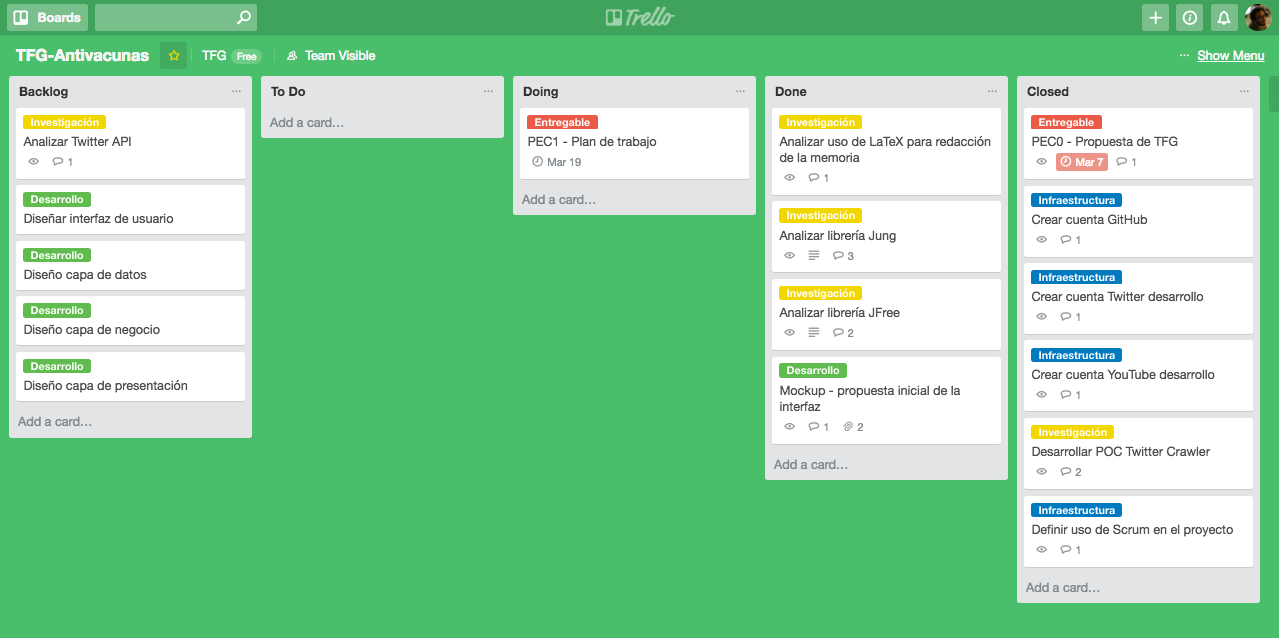
\includegraphics[scale=0.3]{planificacion/trello-backlog.png}
\caption{Ejemplo del backlog del proyecto en Trello}
\end{figure}
\medskip 

\subsection{Planificación del Trabajo}
En la realización del proyecto se propuso inicialmente seguir una planificación tentativa tal y como se detalla en el diagrama de \textit{Grantt} facilitado en las figuras dos y tres:

\begin{figure}[H]
\centering
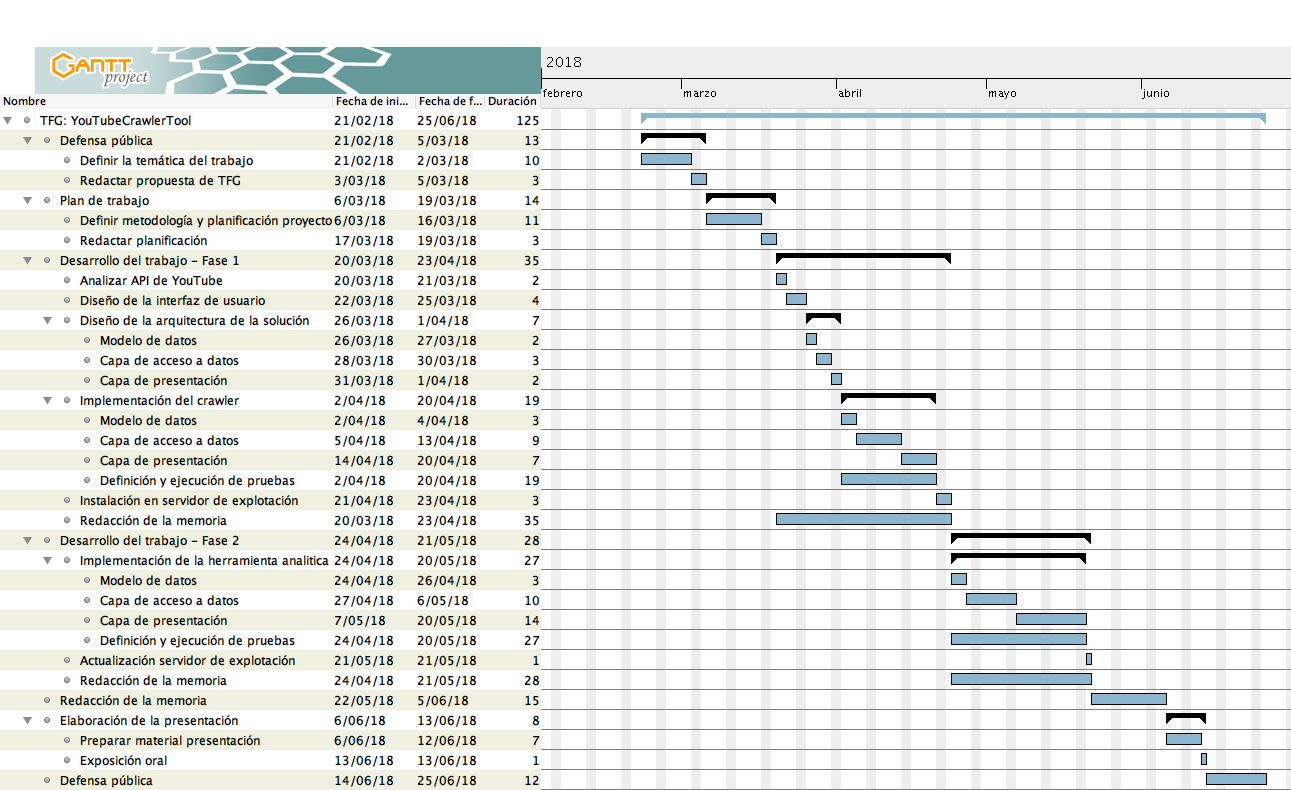
\includegraphics[scale=0.25]{planificacion/planificacion.png}
\caption{Listado de tareas y diagrama de Gantt}
\end{figure}

\begin{figure}[H]
\centering
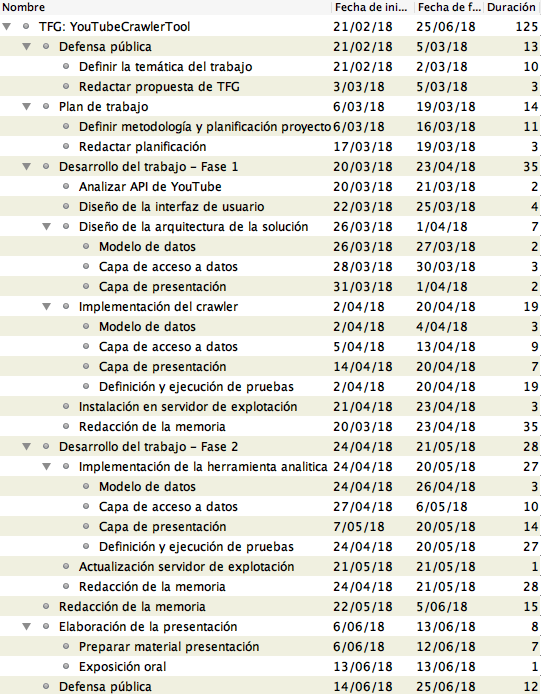
\includegraphics[scale=0.4]{planificacion/listado-tareas.png}
\caption{Listado de tareas}
\end{figure}
\newpage

De la planificación inicial cabe destacar que la redacción de la memoria se diseño como una tarea evolutiva que se desarrollaría durante todas las fases del proyecto pero mas intensamente durante la antepenúltima fase dedicada exclusivamente a su redacción. Además, durante las dos fases de desarrollo se  planificaron dos tareas recurrentes para la definición y realización de pruebas de calidad del producto a realizar durante todo el ciclo de desarrollo.
\\

Como se puede observar, en el diagrama facilitado en cada entrega se pretendían conseguir unos hitos concretos. La relación de los mas destacables por entrega son los siguientes:

\begin{itemize}
\item \textbf{Definición de los contenidos del trabajo:} Redacción propuesta TFG.
\item \textbf{Plan de trabajo:} Redacción planificación.
\item \textbf{Desarrollo del trabajo – Fase 1:} Instalación en servidor de explotación de la primera versión de la aplicación con funcionalidad de \textit{crawler} implementada.
\item \textbf{Desarrollo del trabajo – Fase 2:} Actualización en servidor de explotación de la versión final de la aplicación con funcionalidad analítica implementada.
\item \textbf{Redacción de la memoria:} Entrega de la memoria del proyecto.
\item \textbf{Elaboración de la presentación:} Realizar exposición oral.
\item \textbf{Defensa pública:} Defender públicamente el proyecto.
\end{itemize}

Los riesgos detectados en la planificación inicial se concentraban principalmente en la consecución del hito definido en la primera fase de desarrollo. Para permitir a la clienta de la aplicación poder empezar a recopilar datos para su investigación lo antes posible, se decidió realizar la instalación de la aplicación desarrollada en un entorno de explotación en dos fases distintas, una con la funcionalidad del \textit{crawler} y otra con la funcionalidad analítica implementada. La demora en la primera fase de desarrollo podría comprometer el éxito de la investigación del cliente. Para mitigar este riesgo se realizo el seguimiento del mismo durante las diferentes iteraciones en esa fase de desarrollo. 
\\

Cabe destacar que el diagrama proporcionado en esta sección representa la estimación inicial de la planificación del proyecto de forma tentativa y fue sujeto a modificaciones al inicio de cada nueva fase de desarrollo para garantizar el éxito del proyecto. En la sección de conclusiones del presente documento en el apartado \ref{sec:seguiminetoPlanificacion} se realiza una comparación entre la planificación inicial y sus respectivas revisiones.
\newpage


\subsection{Arquitectura tecnológica}
Para la consecución de los objetivos definidos se ha desarrollado una aplicación web bautizada como \textit{YouTubeCrawlerTool} la cual ha sido diseñada por capas.
\\

La capa de negocio de dicha aplicación ha sido desarrollada con tecnología Java EE \cite{10} implementada mayormente utilizando proyectos del marco de desarrollo Spring Framework \cite{11} entre otros. En esta capa se hace uso intensivo de servicios externos en forma de API pública ofrecida por YouTube con el fin de consumir dicha API para recolectar los vídeos requeridos por el usuario para su estudio.
\\

En la capa de presentación se ha utilizado el lenguaje JavaScript \cite{12} con un gran uso de JQuery \cite{13} para modificar el DOM de las vistas y realizar llamadas asíncronas a la API Rest habilitada en la capa de negocio para tales efectos.
\\

Finalmente, en la capa de datos se utiliza una base de datos orientada a grafos \cite{14} la cual nos permite persistir los vídeos obtenidos en forma de grafo junto con sus relaciones ademas de otras informaciones derivadas y necesarias para el uso y funcionamiento de la aplicación.
\\

En los siguientes apartados se profundiza en la arquitectura y el diseño de la aplicación introducidos en esta sección.
\medskip 

\subsection{Resumen de capítulos}
En los próximos capítulos se detalla el trabajo realizado juntamente con los productos obtenidos y sus conclusiones. La relación de capítulos es la siguiente:

\begin{itemize}
\item \textbf{Análisis y diseño:} Explicación de la metodología de diseño escogida así como los pasos que se llevaron a cabo para definir una propuesta a la clienta y su posterior análisis para acabar definiendo la arquitectura de la solución.
\item \textbf{Desarrollo:} Descripción del desarrollo efectuado y de las decisiones realizadas durante el proceso.
\item \textbf{Implementación y puesta en funcionamiento:} Detalle de los productos obtenidos con las instrucciones para su correcta puesta en funcionamiento ademas de las acciones de formación realizadas.
\item \textbf{Conclusiones:} Sumario de resultados obtenidos y conclusiones sobre el trabajo realizado.
\end{itemize}

\newpage 



\section{Análisis y diseño}
\bigskip 

\subsection{Metodología}\label{metodologia} 
Para realizar el diseño de la aplicación se opto de entre diferentes posibilidades el enfoque definido por la filosofía del 'Diseño centrado en el usuario' \cite{15}.
\\

El diseño centrado en el usuario, como bien indica su nombre, se caracteriza por conocer a fondo a los futuros usuarios de una aplicación para diseñar un producto que resuelva sus necesidades y expectativas buscando en todo momento conseguir la mayor satisfacción del usuario posible. Se trata de un proceso iterativo y cíclico por fases en donde en cada una de ellas se utilizan distintas técnicas para conseguir los objetivos propuestos. 
\\

En nuestro proyecto se ha decidido seguir esta y no otra metodología de diseño tales como el 'Diseño centrado en la actividad' o el 'Diseño centrado en el uso' debido a que, como en nuestro caso la clienta de la aplicación va a ser también la usuaria final de la misma, se ha decidido realizar el análisis de la aplicación centrada en ella y sus necesidades por encima de la actividad que se llevara a cabo o el uso.
\\

La relación de fases y técnicas utilizadas ha sido la siguiente:

\begin{itemize}
\item \textbf{Definir contexto de uso:} El objetivo de esta fase es el de determinar que necesidades pretende la usuaria final que la aplicación resuelva y a que se va a destinar su uso. La técnica escogida para la realización de esta fase fueron las entrevistas con la usuaria final que se realizaron mediante videoconferencia sobretodo durante las diferentes \textit{sprint reviews} al termino de cada \textit{sprint}.
\item \textbf{Especificar requisitos:} En la siguiente fase se definen los requisitos del sistema a partir de la información recogida en la fase previa. Para los requisitos funcionales se opto por recogerlos como 'casos de uso' \cite{16}.
\item \textbf{Diseñar el producto:} En esta fase se diseñan y implementan los requisitos definidos en la fase anterior ya sea con el objetivo de proporcionar una solución final o una propuesta de solución a ser refinada en sucesivas iteraciones. Las técnicas utilizadas en esta fase fueron la creación de maquetas para evaluar la solución y el prototipado mediante pruebas de concepto realizadas con el objetivo de estudiar posibles soluciones antes de realizar su implementación en la aplicación.
\item \textbf{Poner a prueba el producto:} Finalmente, en esta fase se pone a prueba el producto obtenido. Para hacerlo, se definieron y ejecutaron pruebas de integración diseñadas teniendo en cuenta los casos de uso definidos previamente y se realizaron test con usuarios para evaluar su grado de satisfacción.
\end{itemize}

Gracias al enfoque escogido fue posible encontrar respuestas a preguntas sobre las expectativas que la usuaria tenia depositadas sobre la aplicación y que fueron de gran ayuda a la hora de diseñar la solución final. Algunas de las principales preguntas fueron:\\
\textit{¿Quiénes son los usuarios de la aplicación?}\\
\textit{¿Cuáles son las tareas a realizar?}\\
\textit{¿Qué funcionalidades se necesitan?}\\
\textit{¿Qué información se necesita?}
\\

También cabe destacar que gracias a que tanto \textit{scrum} como el diseño centrado en el usuario son dos procesos iterativos, resulto fácil integrar esta metodología dentro del marco ágil de desarrollo.
\medskip 

\subsection{Propuesta de la solución}
\medskip 

\subsubsection{Reuniones y entrevistas}
Tal y como se ha introducido en la sección \ref{metodologia} sobre la metodología de diseño utilizada, para definir el contexto de uso y conocer las necesidades a ser cubiertas por la aplicación, se realizaron varias entrevistas con la clienta y los \textit{stakeholders} donde la gran mayoría de ellas fueron dentro del contexto de \textit{scrum} como reuniones de \textit{sprint review} y \textit{sprint planning}.
\\

A continuación se resumen las entrevistas y reuniones realizadas junto con los principales temas tratados y decisiones tomadas:
\\

\noindent\textbf{Fecha:} 05/03/2018
\\
\noindent\textbf{Hora de inicio:} 21:00
\\
\noindent\textbf{Hora final:} 21:45
\\
\noindent\textbf{Asistentes:} 
\begin{itemize}
\item Carlos Luis Sánchez Bocanegra: \textit{stakeholder}
\item Johanna Milena Rodríguez Vera: clienta
\item Javier Sánchez Mendoza: \textit{product owner}, \textit{scrum master} y desarrollador
\end{itemize}
\noindent\textbf{Temas tratados:}
\begin{itemize}
\item Que conocimiento sobre el movimiento antivacunas se quiere obtener. 
\item Que se pretende hacer con la información recolectada.
\item Definición de los objetivos de la aplicación.
\end{itemize}
\noindent\textbf{Decisiones:}
\begin{itemize}
\item La clienta definirá los criterios de búsqueda y el conocimiento que debe ser obtenido por la aplicación.
\item El análisis de los datos los realizara la clienta con herramientas especializadas.
\item El objetivo principal de la aplicación es la obtención de datos mediante búsquedas en redes sociales.
\item La aplicación debe ofrecer funcionalidad para exportar los datos recolectados a otras herramientas.
\end{itemize}

\begin{center}\rule{10cm}{0.4pt}\end{center}

\noindent\textbf{Fecha:} 12/03/2018
\\
\noindent\textbf{Hora de inicio:} 21:00
\\
\noindent\textbf{Hora final:} 21:30
\\
\noindent\textbf{Asistentes:} 
\begin{itemize}
\item Carlos Luis Sánchez Bocanegra: \textit{stakeholder}
\item Johanna Milena Rodríguez Vera: clienta
\item Javier Sánchez Mendoza: \textit{product owner}, \textit{scrum master} y desarrollador
\end{itemize}
\noindent\textbf{Temas tratados:}
\begin{itemize}
\item Alcance del estudio a realizar.
\item Sobre que redes sociales debe centrarse el estudio.
\end{itemize}
\noindent\textbf{Decisiones:}
\begin{itemize}
\item Se decide adoptar el marco de trabajo \textit{scrum} para la realización del proyecto.
\item El estudio se centrara inicialmente en una sola red social a determinar.
\item En la aplicación sera posible ejecutar varios procesos de recolección de datos al mismo tiempo.
\item Se incorporara una sección para analizar los datos obtenidos de forma visual (por definir).
\item El \textit{product owner} realizara una propuesta inicial de la interfaz de usuario.
\end{itemize}

\begin{center}\rule{10cm}{0.4pt}\end{center}

\noindent\textbf{Fecha:} 19/03/2018
\\
\noindent\textbf{Hora de inicio:} 21:00
\\
\noindent\textbf{Hora final:} 21:30
\\
\noindent\textbf{Asistentes:} 
\begin{itemize}
\item Carlos Luis Sánchez Bocanegra: \textit{stakeholder}
\item Johanna Milena Rodríguez Vera: clienta
\end{itemize}
\noindent\textbf{Temas tratados:}
\begin{itemize}
\item Comentarios sobre la propuesta inicial de la interfaz de usuario realizada por el \textit{product owner}.
\item Pros y contras sobre la elección de \textit{Twitter} como red social para el estudio.
\end{itemize}
\noindent\textbf{Decisiones:}
\begin{itemize}
\item Elección de \textit{Twitter} como red social a utilizar en el estudio.
\item La aplicación incluirá una visualización en forma de grafo para poder analizar visualmente las relaciones existente en la información recolectada y descubrir patrones.
\item El \textit{product owner} debe estudiar la viabilidad de utilizar \textit{Twitter} para la consecución de los objetivos. 
\end{itemize}

\begin{center}\rule{10cm}{0.4pt}\end{center}

\noindent\textbf{Fecha:} 26/03/2018
\\
\noindent\textbf{Hora de inicio:} 21:00
\\
\noindent\textbf{Hora final:} 21:45
\\
\noindent\textbf{Asistentes:} 
\begin{itemize}
\item Carlos Luis Sánchez Bocanegra: \textit{stakeholder}
\item Johanna Milena Rodríguez Vera: clienta
\end{itemize}
\noindent\textbf{Temas tratados:}
\begin{itemize}
\item Debido a las limitaciones de uso detectadas en la API de \textit{Twitter}, se propone utilizar la red social \textit{YouTube} como alternativa.
\item Definición del grafo a utilizar y que elementos actuaran como nodo y aristas.  
\end{itemize}
\noindent\textbf{Decisiones:}
\begin{itemize}
\item Elección de \textit{YouTube} como red social a utilizar en el estudio.
\item El \textit{product owner} debe estudiar la viabilidad de utilizar \textit{YouTube} para la consecución de los objetivos. 
\item Actualizar la propuesta de interfaz de usuario para reflejar el cambio de red social.
\end{itemize}

\begin{center}\rule{10cm}{0.4pt}\end{center}

\noindent\textbf{Fecha:} 05/04/2018
\\
\noindent\textbf{Hora de inicio:} 21:00
\\
\noindent\textbf{Hora final:} 21:45
\\
\noindent\textbf{Asistentes:} 
\begin{itemize}
\item Carlos Luis Sánchez Bocanegra: \textit{stakeholder}
\item Johanna Milena Rodríguez Vera: clienta
\item Javier Sánchez Mendoza: \textit{product owner}, \textit{scrum master} y desarrollador
\end{itemize}
\noindent\textbf{Temas tratados:}
\begin{itemize}
\item Comentarios sobre la propuesta inicial de la interfaz de usuario realizada por el \textit{product owner}.
\item Analizar criterios de búsqueda y información devuelta por la API de \textit{YouTube}
\item Detección de vídeos duplicados.
\item Detectar usuarios \textit{influencers} a partir de la información obtenida.
\item Avances en la definición de los componentes del grafo.
\end{itemize}
\noindent\textbf{Decisiones:}
\begin{itemize}
\item Criterios de búsqueda de \textit{YouTube} a utilizar para recolectar los vídeos.
\item Campos a almacenar de cada vídeo.
\item Incorporar funcionalidad para ver resumen de las búsquedas realizadas junto con la información recolectada con pre visualización de vídeos.
\item Utilizar una variable pre calculada (bautizada como "\textit{scopeRange}") para determinar el tamaño de los nodos al ser visualizados en el grafo.
\end{itemize}

\begin{center}\rule{10cm}{0.4pt}\end{center}

\noindent\textbf{Fecha:} 12/04/2018
\\
\noindent\textbf{Hora de inicio:} 21:30
\\
\noindent\textbf{Hora final:} 22:15
\\
\noindent\textbf{Asistentes:} 
\begin{itemize}
\item Carlos Luis Sánchez Bocanegra: \textit{stakeholder}
\item Johanna Milena Rodríguez Vera: clienta
\item Javier Sánchez Mendoza: \textit{product owner}, \textit{scrum master} y desarrollador
\end{itemize}
\noindent\textbf{Temas tratados:}
\begin{itemize}
\item Comentarios sobre la visualización en grafo.
\item Identificación de vídeos pro y anti vacunación.
\end{itemize}
\noindent\textbf{Decisiones:}
\begin{itemize}
\item Queda definida la visualización en grafo.
\item Los contenidos a visualizar en el grafo podrán ser filtrados.
\item Se define funcionalidad para etiquetar los vídeos recolectados utilizando categorías previamente definidas por el usuario en la aplicación.
\item En la aplicación habrá dos tipos de usuarios, usuarios anónimos que no podrán realizar acciones de escritura ni borrado y usuarios registrados que podrán realizar todas la acciones.
\item Incorporar visualizaciones estadísticas sobre el uso de las categorías.
\item Realización de una ultima propuesta de interfaz de usuario que recoja los últimos cambios propuestos junto con la visualización en grafo.
\end{itemize}

\begin{center}\rule{10cm}{0.4pt}\end{center}

\noindent\textbf{Fecha:} 19/04/2018
\\
\noindent\textbf{Hora de inicio:} 21:30
\\
\noindent\textbf{Hora final:} 22:00
\\
\noindent\textbf{Asistentes:} 
\begin{itemize}
\item Carlos Luis Sánchez Bocanegra: \textit{stakeholder}
\item Johanna Milena Rodríguez Vera: clienta
\item Javier Sánchez Mendoza: \textit{product owner}, \textit{scrum master} y desarrollador
\end{itemize}
\noindent\textbf{Temas tratados:}
\begin{itemize}
\item Comentarios sobre la propuesta de interfaz de usuario. 
\item Priorización de funcionalidades.
\end{itemize}
\noindent\textbf{Decisiones:}
\begin{itemize}
\item La clienta da por aprobada la propuesta de interfaz de usuario.
\item Definición de valores por defecto al realizar las búsquedas de contenidos.
\item Las funcionalidades estadísticas y de visualización de canales quedan asignadas con una prioridad secundaria en relación a otras funcionalidades.
\item Se va a buscar la colaboración de un estadista para definir la formula de la variable "\textit{scopeRange}".
\end{itemize}

\begin{center}\rule{10cm}{0.4pt}\end{center}

\noindent\textbf{Fecha:} 26/04/2018
\\
\noindent\textbf{Hora de inicio:} 21:00
\\
\noindent\textbf{Hora final:} 21:30
\\
\noindent\textbf{Asistentes:} 
\begin{itemize}
\item Carlos Luis Sánchez Bocanegra: \textit{stakeholder}
\item Johanna Milena Rodríguez Vera: clienta
\item Javier Sánchez Mendoza: \textit{product owner}, \textit{scrum master} y desarrollador
\end{itemize}
\noindent\textbf{Temas tratados:}
\begin{itemize}
\item Seguimiento de la implementación de la aplicación
\item Seguimiento de la definición de la fórmula para calcular el alcance de los vídeos ("\textit{scopeRange}").
\end{itemize}
\noindent\textbf{Decisiones:}

\begin{center}\rule{10cm}{0.4pt}\end{center}

\noindent\textbf{Fecha:} 03/05/2018
\\
\noindent\textbf{Hora de inicio:} 21:00
\\
\noindent\textbf{Hora final:} 21:30
\\
\noindent\textbf{Asistentes:} 
\begin{itemize}
\item Carlos Luis Sánchez Bocanegra: \textit{stakeholder}
\item Johanna Milena Rodríguez Vera: clienta
\item Javier Sánchez Mendoza: \textit{product owner}, \textit{scrum master} y desarrollador
\end{itemize}
\noindent\textbf{Temas tratados:}
\begin{itemize}
\item Seguimiento de la implementación de la aplicación.
\item Seguimiento de la definición de la fórmula para calcular el alcance de los vídeos ("\textit{scopeRange}").
\end{itemize}
\noindent\textbf{Decisiones:}

\begin{center}\rule{10cm}{0.4pt}\end{center}

\noindent\textbf{Fecha:} 10/05/2018
\\
\noindent\textbf{Hora de inicio:} 20:30
\\
\noindent\textbf{Hora final:} 21:00
\\
\noindent\textbf{Asistentes:} 
\begin{itemize}
\item Carlos Luis Sánchez Bocanegra: \textit{stakeholder}
\item Johanna Milena Rodríguez Vera: clienta
\item Javier Sánchez Mendoza: \textit{product owner}, \textit{scrum master} y desarrollador
\end{itemize}
\noindent\textbf{Temas tratados:}
\begin{itemize}
\item Seguimiento de la implementación de la aplicación.
\item Seguimiento de la definición de la fórmula para calcular el alcance de los vídeos ("\textit{scopeRange}").
\end{itemize}
\noindent\textbf{Decisiones:}
\begin{itemize}
\item Instalación de la aplicación en entorno de explotación durante la próxima semana.
\item Mientras no se disponga de la formula para la variable "\textit{scopeRange}", utilizar formula alternativa definida por la clienta.
\end{itemize}

\begin{center}\rule{10cm}{0.4pt}\end{center}

\noindent\textbf{Fecha:} 17/05/2018
\\
\noindent\textbf{Hora de inicio:} 20:30
\\
\noindent\textbf{Hora final:} 21:30
\\
\noindent\textbf{Asistentes:} 
\begin{itemize}
\item Carlos Luis Sánchez Bocanegra: \textit{stakeholder}
\item Johanna Milena Rodríguez Vera: clienta
\item Javier Sánchez Mendoza: \textit{product owner}, \textit{scrum master} y desarrollador
\end{itemize}
\noindent\textbf{Temas tratados:}
\begin{itemize}
\item Presentación de la aplicación desarrollada y formación a la clienta.
\end{itemize}
\noindent\textbf{Decisiones:}
\begin{itemize}
\item Se decide utilizar la formula alternativa propuesta por la clienta para la variable "\textit{scopeRange}".
\item Añadir nueva funcionalidad de favoritos.
\item Realización de cambios en la visualización de los listados de los vídeos.
\end{itemize}

\begin{center}\rule{10cm}{0.4pt}\end{center}

En los siguientes apartados se detallan algunas de las decisiones tomadas en estas reuniones las cuales tuvieron mas repercusión en el resultado final de la aplicación.
\medskip 

\subsubsection{Elección de YouTube como red social}
A la hora de escoger una red social para realizar el estudio del movimiento antivacuna nos encontramos con una gran variedad de opciones, tales como \textit{Facebook}, \textit{Twitter} o \textit{YouTube} para nombrar solo algunas.
\\

Johanna, clienta de la aplicación y la encargada de realizar el estudio, mostró su predilección inicial por \textit{Twitter}. En su criterio, \textit{Twitter} presentaba una estructuración de la información que favorecía su posterior análisis y estudio al basarse, principalmente, un mensaje (\textit{tweet}) de los campos titulo y descripción, hecho que facilitaba la categorización de los contenidos obtenidos. Por otro lado, el uso extensivo de etiquetas en esta red social (\textit{hashtags}) simplificaría el proceso de búsqueda de contenidos. Por lo referente al alcance de la red social, Johanna consideraba que a nivel de usuarios y actividad relacionada con la vacunación, \textit{Twitter} superaba a otras redes sociales tales como \textit{YouTube}.
\\

Debido a estas consideraciones, \textit{Twitter} fue escogida inicialmente como la red social a utilizar en el proyecto. Por este motivo, inicialmente la aplicación desarrollada se llamaba \textit{TwitterCrawlerTool} y las primeras versiones de la propuesta de interfaz de usuario se habían realizado teniendo en consideración a \textit{Twitter} como red social escogida. Incluso, una prueva de concepto llego a desarrollarse: \href{https://github.com/jsanchezmend/TFGAntivacunas/tree/master/POCTwitterCrawler}{POCTwitterCrawler}.
\\

Con la elección realizada y teniendo desarrollada una prueba de concepto, se procedió al estudio en profundidad de la API de \textit{Twitter} y fue entonces cuando se descubrieron limitaciones sobre su uso. Concretamente, \textit{Twitter} define tres niveles de uso: \textit{Standard}, \textit{Premium} y \textit{Enterprise}; de todas ellas solo la opción \textit{Standard} es completamente gratuita pero, en este caso, con unas severas restricciones de uso a la hora de buscar mensajes \cite{17}. Algunas de las restricciones son:
\begin{itemize}
\item Máximo de 100 \textit{"tweets"} por búsqueda.
\item Información disponible solo de los últimos 7 días.
\item Solo permite búsqueda textual, no se permite búsqueda temporal.
\end{itemize}

A causa de estas restricciones, resultaba imposible poder recabar información con una antigüedad inferior a siete días o realizar comparaciones en el tiempo sobre la evolución de los movimientos pro y anti vacunas, hecho que es requerido en el estudio. Ante los descubrimientos realizados se decidió explorar otras alternativas al uso de \textit{Twitter}.
\\

Fue entonces que la opción de utilizar \textit{YouTube} como red social de estudio en el proyecto se considero en profundidad. Y es que aunque se llegara anteriormente a la conclusión de que \textit{Twitter} tenia un alcance mayor en numero de usuarios y potencial de contenidos a obtener, no se debe desestimar tampoco el alcance de \textit{YouTube} que, si bien inicialmente no era considerada como una red social al uso, a día de hoy el numero de usuarios que no solo visualizan sus vídeos sino que también comparten contenidos y comentarios crece día a día, convirtiendo a \textit{YouTube} como una buena opción para encontrar la información requerida. Y en lo referente a la estructuración de la información, debido a que juntamente con los vídeos se provee un titulo y una descripción no era necesario cambiar el enfoque dado inicialmente en este sentido.
\\

Por lo referente a la API ofrecida por \textit{YouTube} para la obtención de contenidos, los criterios de búsqueda disponibles son mucho mas amplios que los ofrecidos por \textit{Twitter}, permitiéndonos entre otras posibilidades, filtrar los contenidos a obtener por rangos de fechas. No existe limitación a la hora de obtener contenidos independientemente de su fecha de publicación (en todo caso posterior a 14/02/2005, fecha de fundación de \textit{YouTube}). Y en relación a limitaciones en el volumen de información a obtener, \textit{YouTube} no impone limitaciones por búsqueda, lo que posibilita obtener toda la información requerida sobre un termino en concreto. En su defecto, \textit{YouTube} utiliza un sistema de cuotas que se aplica a periodos de tiempo en concreto \cite{18}, por ejemplo, en su versión gratuita permite realizar hasta 1.000.000 de operaciones de lectura por día que, tal y como se ha demostrado, han sido suficientes para el uso dado a la aplicación desarrollada. Para estudiar su viabilidad en el proyecto, se realizo una prueba de concepto con resultados satisfactorios: \href{https://github.com/jsanchezmend/TFGAntivacunas/tree/master/POCYouTubeCrawler}{POCYouTubeCrawler}.
\\

En el apartado \ref{youTubeDataAPI} se detalla en profundidad los servicios de la API de \textit{YouTube} utilizados y el modo en que la aplicación los consume para obtener contenidos. 
\medskip 

\subsubsection{Visualización de vídeos en grafo}
Otra de las decisiones de diseño mas debatidas fue la definición de una vista en la aplicación que permitiera de forma visual analizar como se relacionan los movimientos anti y pro vacuna en la red social de \textit{YouTube}. 
\\

La motivación principal de la misma es la de proporcionar una funcionalidad con la cual fuera posible estudiar las vías de acceso a los contenidos y observar que movimiento tiene mas alcance de audiencia en \textit{YouTube}. Para tales efectos, se llego a la conclusión que una visualización en formato de grafo donde fuera posible distinguir los dos movimientos a estudio seria la forma mas efectiva de representar dicha información.
\\

Para difinir el grafo, necesitábamos analizar que componentes actuarían como nodo y que representarían las aristas entre ellos, ademas de tomar otras decisiones como si se incorporarían pesos al grafo y si este seria dirigido o no. Para ayudar en la definición del grafo, se realizaron propuestas que se apoyaron con pruebas realizadas manualmente por parte de la clienta con contenidos reales:

\begin{figure}[H]
\centering
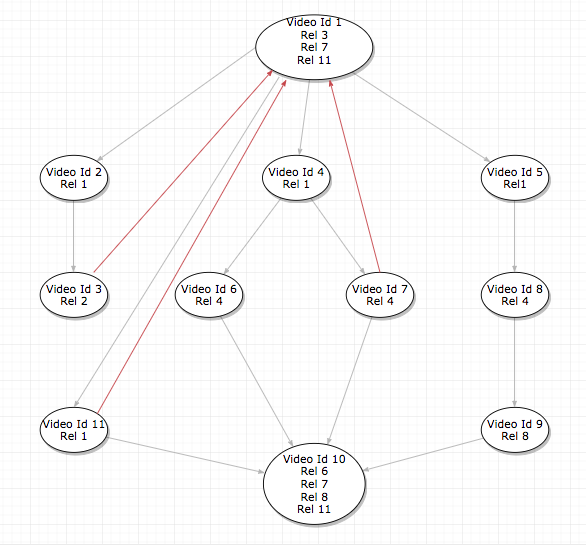
\includegraphics[scale=0.40]{grafo/propuesta1.png}
\caption{Propuesta grafo dirigido}
\end{figure}

\begin{figure}[H]
\centering
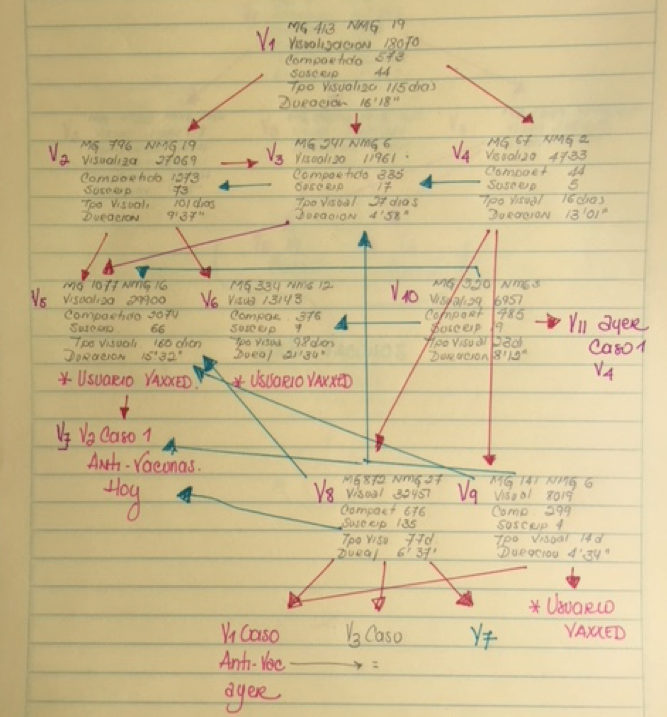
\includegraphics[scale=0.40]{grafo/pruebaManual.png}
\caption{Maqueta de grafo dirigido}
\end{figure}
\bigskip 

Como conclusiones del análisis realizado se definió el grafo a representar con las siguientes características:
\begin{itemize}
\item \textbf{Tipo:} Grafo dirigido sin pesos.
\item \textbf{Nodos:} Vídeos y canales (canales de forma opcional).
\item \textbf{Aristas:} Entre dos vídeos representa que desde el vídeo origen es posible acceder al vídeo destino (mediante la recomendación realizada por \textit{YouTube} como vídeos relacionados). Y entre un vídeo y un canal representa que el vídeo (nodo origen) ha sido publicado por el canal relacionado (nodo destino).
\item \textbf{Visualización:} En nodos tipo vídeo, su tamaño sera determinado por su alcance de audiencia y el color de representación sera determinado por su categoría (anti o pro vacuna). En el caso de nodos tipo canal su tamaño y representación no sera determinado por ninguna de sus características, por lo que todos los canales se visualizaran con el mismo formato pero diferenciados de los nodos tipo vídeo. Sera posible ver una pre visualización del contenido al hacer clic en el.
\end{itemize}

Para estudiar su viabilidad, se realizo una prueba de concepto con resultado favorable: \href{https://github.com/jsanchezmend/TFGAntivacunas/tree/master/POCYouTubeCrawler}{POCYouTubeCrawler}.
\begin{figure}[H]
\centering
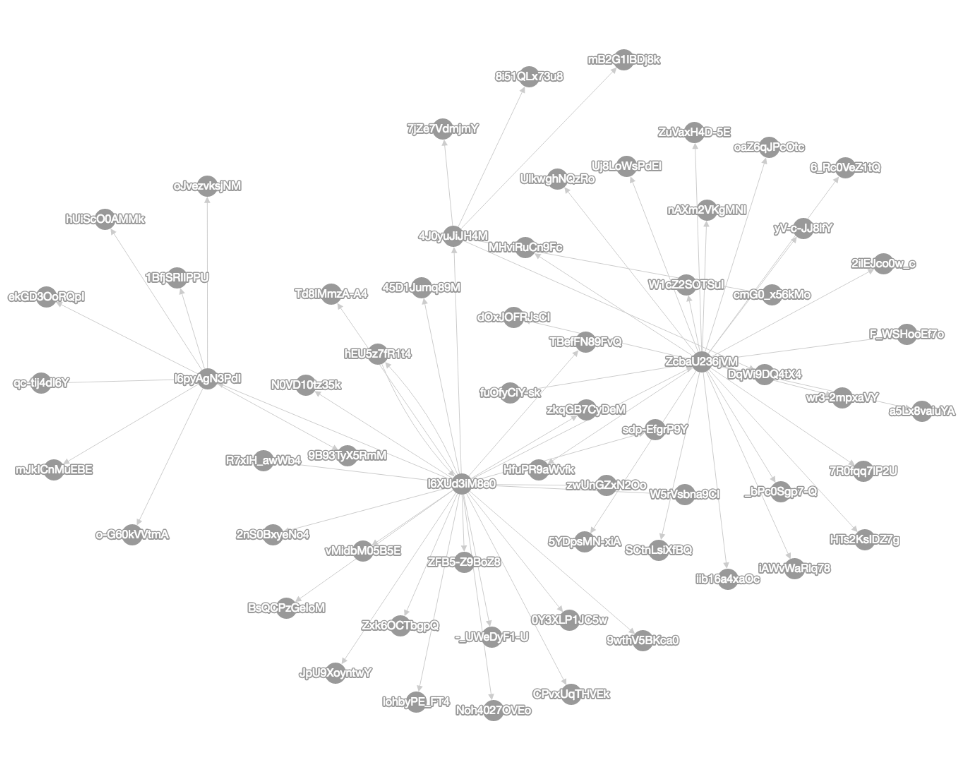
\includegraphics[scale=0.30]{grafo/pocGrafo.png}
\caption{Prueba de concepto de grafo dirigido}
\end{figure}

En la propuesta de grafo detallada, se detectaron dos requerimientos encubiertos necesarios para su realización: la necesidad de categorizar vídeos y la definición de una variable que nos permitiera determinar el alcance de audiencia de un vídeo para definir su tamaño en el grafo.
\\

Para la categorización de los vídeos, se diseño una funcionalidad genérica que permitiera al usuario definir las categorías necesarias con las cuales posteriormente poder etiquetar los vídeos. El inconveniente de esta solución es que para poder visualizar correctamente el grafo y identificar los grupos de nodos, se requiere realizar previamente una tarea de categorización manual de los vídeos. Después de analizar la problemática, debido a que el volumen de datos requeridos para realizar el estudio se determino en una cifra menor a mil, se acepto la solución como viable pero, en este caso, se debía tener presente esta circunstancia en la planificación del proyecto.
\\

Por otro lado, para definir el tamaño de visualización del nodo se estudio la creación de una variable apodada como \textit{scopeRange}. Dicha variable, debía representar dentro de un rango de valores valido, el alcance o popularidad obtenido por un vídeo en concreto. Para ello se estudio poder identificar a los usuarios mas influyentes de \textit{YouTube} (conocidos como \textit{influencers}), pero finalmente se decidió utilizar la información estadística ofrecida por \textit{YouTube} para cada vídeo, la cual se compone de los campos:
\begin{itemize}
\item \textbf{\textit{viewCount}:} Numero de visualizaciones del vídeo.
\item \textbf{\textit{likeCount}:} Numero de personas a las cuales le ha gustado el vídeo.
\item \textbf{\textit{dislikeCount}:} Numero de personas a las cuales no le ha gustado el vídeo.
\item \textbf{\textit{commentCount}:} Numero de comentario que ha recibido el vídeo.
\end{itemize}

Para la definición de la formula se pidió la colaboración de un estadista. Pero debido a que la fecha final de desarrollo del proyecto se aproximaba y aun no se disponía de la colaboración, se opto por aplicar una formula definida por la clienta que en las pruebas realizadas demostró efectividad:
\begin{center}
$$scopeRange = \frac{likeCount}{dislikeCount}$$
\end{center}
Con un valor mínimo definido de 10 para asegurar la visualización del vídeo en el grafo.
\\

A modo ilustrativo, a continuación se adjunta una imagen de la implementación del grafo en la aplicación:
\begin{figure}[H]
\centering
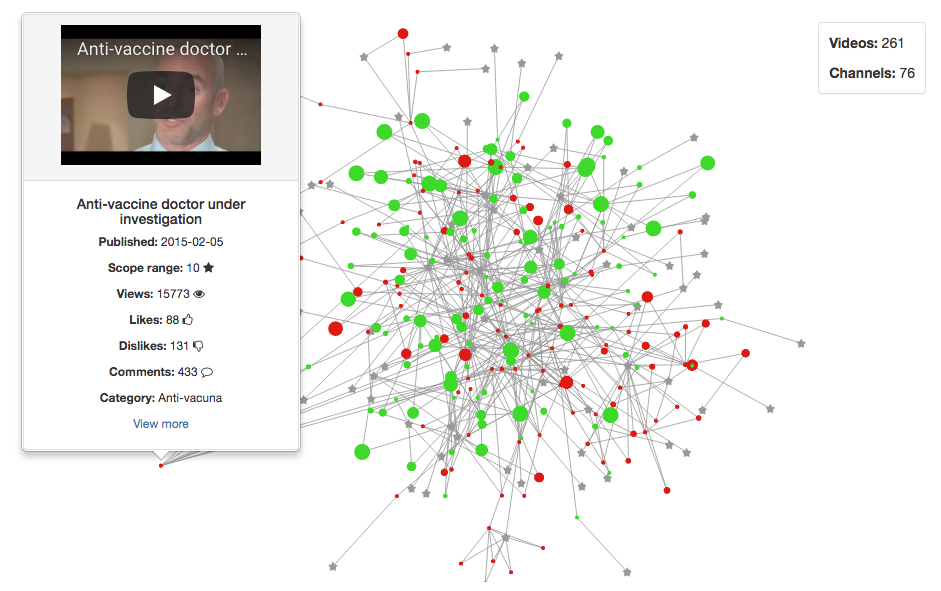
\includegraphics[scale=0.40]{grafo/final.png}
\caption{Implementación del grafo en la aplicación}
\end{figure}
\medskip 

\subsubsection{Casos de uso}
Hacer uso de un marco ágil de desarrollo no debe ser escusa para no disponer de una documentación adecuada de los requisitos de una aplicación y, aunque estos sufran modificaciones durante las diferentes iteraciones de desarrollo, estos deben de estar actualizados. Por esta razón se ha decidido realizar la toma de requerimientos de la aplicación en forma de casos de uso, en donde para facilitar la gestión de cambios se ha decidido hacer constar solo el titulo, actores y descripción en cada uno de ellos.
\\

Así entonces y con lo expuesto en apartados anteriores, a continuación se expone una imagen representativa de los casos de uso identificados agrupados por componentes según la funcionalidad realizada y a continuación el listado completo de cada uno de ellos:

\begin{figure}[H]
\centering
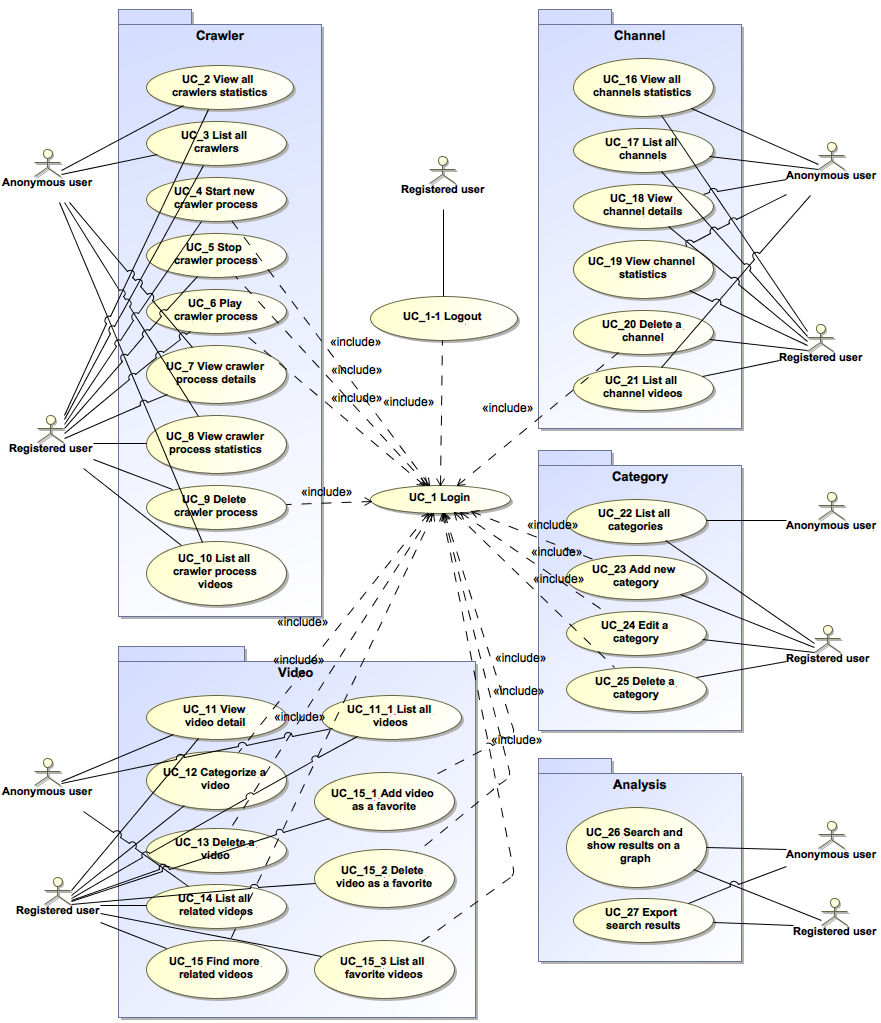
\includegraphics[scale=0.35]{requisitos/UseCases.png}
\caption{Casos de uso}
\end{figure}
\medskip 
\medskip 

\noindent\textbf{Componente \textit{User session}:}
\\

\noindent\textbf{UC\_1: Login}\\
\textbf{Actores:} Usuario anónimo\\
\textbf{Descripción:} Como usuario anónimo, quiero identificarme en la aplicación mediante nombre de usuario y contraseña.
\\

\noindent\textbf{UC\_1-1: logout}\\
\textbf{Actores:} Usuario registrado\\
\textbf{Descripción:} Como usuario identificado, quiero cerrar la sesión actual en la aplicación.
\\

\begin{center}\rule{10cm}{0.4pt}\end{center}

\noindent\textbf{Componente \textit{Crawler}:}
\\

\noindent\textbf{UC\_2: View all crawlers statistics}\\
\textbf{Actores:} Usuario anónimo, Usuario registrado\\
\textbf{Descripción:} Como usuario, quiero ver el total de vídeos recolectados, el porcentaje de categorizados y la distribución de las categorías.
\\

\noindent\textbf{UC\_3: List all crawlers}\\
\textbf{Actores:} Usuario anónimo, Usuario registrado\\
\textbf{Descripción:} Como usuario, quiero ver todos los procesos de recolección que se han iniciado en el sistema.
\\

\noindent\textbf{UC\_4: Start new crawler process}\\
\textbf{Actores:} Usuario registrado\\
\textbf{Descripción:} Como usuario identificado, quiero iniciar un nuevo proceso de recolección de vídeos según criterio de búsqueda introducido.
\\

\noindent\textbf{UC\_5: Stop crawler process}\\
\textbf{Actores:} Usuario registrado\\
\textbf{Descripción:} Como usuario identificado, quiero parar un proceso de recolección de vídeos que este en ejecución.
\\

\noindent\textbf{UC\_6: Play crawler process}\\
\textbf{Actores:} Usuario registrado\\
\textbf{Descripción:} Como usuario identificado, quiero poner en marcha un proceso de recolección previamente detenido.
\\

\noindent\textbf{UC\_7: View crawler process details}\\
\textbf{Actores:} Usuario anónimo, Usuario registrado\\
\textbf{Descripción:} Como usuario, quiero ver el detalle de un proceso de recolección.
\\

\noindent\textbf{UC\_8: View crawler process statistics}\\
\textbf{Actores:} Usuario anónimo, Usuario registrado\\
\textbf{Descripción:} Como usuario, dado un proceso de recolección en concreto quiero ver su total de vídeos recolectados, su porcentaje de categorizados y su distribución de las categorías.
\\

\noindent\textbf{UC\_9: Delete crawler process}\\
\textbf{Actores:} Usuario registrado\\
\textbf{Descripción:} Como usuario identificado, quiero borrar un proceso de recolección en concreto y todos sus vídeos relacionados.
\\

\noindent\textbf{UC\_10: List all crawler process videos}\\
\textbf{Actores:} Usuario anónimo, Usuario registrado\\
\textbf{Descripción:} Como usuario, quiero ver el listado completo de vídeos recolectados por un proceso de recolección en concreto.
\\

\begin{center}\rule{10cm}{0.4pt}\end{center}

\noindent\textbf{Componente \textit{Video}:}
\\

\noindent\textbf{UC\_11-1: List all videos}\\
\textbf{Actores:} Usuario anónimo, Usuario registrado\\
\textbf{Descripción:} Como usuario, quiero ver listados todos los vídeos del sistema.
\\

\noindent\textbf{UC\_11: View video detail}\\
\textbf{Actores:} Usuario anónimo, Usuario registrado\\
\textbf{Descripción:} Como usuario, quiero ver el detalle de un vídeo en concreto.
\\

\noindent\textbf{UC\_12: Categorize a video}\\
\textbf{Actores:} Usuario registrado\\
\textbf{Descripción:} Como usuario identificado, quiero cambiar la categoría asociada a un vídeo en concreto.
\\

\noindent\textbf{UC\_13: Delete a video}\\
\textbf{Actores:} Usuario registrado\\
\textbf{Descripción:} Como usuario identificado, quiero borrar un vídeo en concreto.
\\

\noindent\textbf{UC\_14: List all related videos}\\
\textbf{Actores:} Usuario anónimo, Usuario registrado\\
\textbf{Descripción:} Como usuario, quiero ver listados todos los vídeos relacionados con un  en concreto.
\\

\noindent\textbf{UC\_15: Find more related videos}\\
\textbf{Actores:} Usuario registrado\\
\textbf{Descripción:} Como usuario identificado, quiero iniciar un nuevo proceso de recolección de vídeos para que encuentre vídeos relacionados a un vídeo en concreto.
\\

\noindent\textbf{UC\_15-1: Add a video as a favorite}\\
\textbf{Actores:} Usuario registrado\\
\textbf{Descripción:} Como usuario identificado, quiero añadir un vídeo en concreto al listado de favoritos.
\\

\noindent\textbf{UC\_15-2: Delete a video as a favorite}\\
\textbf{Actores:} Usuario registrado\\
\textbf{Descripción:} Como usuario identificado, quiero eliminar un vídeo en concreto del listado de favoritos.
\\

\noindent\textbf{UC\_15-3: List all favorite videos}\\
\textbf{Actores:} Usuario registrado\\
\textbf{Descripción:} Como usuario identificado, quiero ver el listado de vídeos favoritos.
\\

\begin{center}\rule{10cm}{0.4pt}\end{center}

\noindent\textbf{Componente \textit{Channel}:}
\\

\noindent\textbf{UC\_16: View all channels statistics}\\
\textbf{Actores:} Usuario anónimo, Usuario registrado\\
\textbf{Descripción:} Como usuario, quiero ver el total de canales importados en el sistema.
\\

\noindent\textbf{UC\_17: List all channels}\\
\textbf{Actores:} Usuario anónimo, Usuario registrado\\
\textbf{Descripción:} Como usuario, quiero ver listados todos los canales importado en el sistema.
\\

\noindent\textbf{UC\_18: View channel details}\\
\textbf{Actores:} Usuario anónimo, Usuario registrado\\
\textbf{Descripción:} Como usuario, quiero ver el detalle de un canal en concreto.
\\

\noindent\textbf{UC\_19: View channel statistics}\\
\textbf{Actores:} Usuario anónimo, Usuario registrado\\
\textbf{Descripción:} Como usuario, dado un canal en concreto quiero ver su total de vídeos recolectados, su porcentaje de categorizados y su distribución de las categorías.
\\

\noindent\textbf{UC\_20: Delete a channel}\\
\textbf{Actores:} Usuario registrado\\
\textbf{Descripción:} Como usuario identificado, quiero eliminar un canal en concreto y todos sus vídeos relacionados.
\\

\noindent\textbf{UC\_21: List all channel videos}\\
\textbf{Actores:} Usuario anónimo, Usuario registrado\\
\textbf{Descripción:} Como usuario, dado un canal en concreto quiero ver listados todos sus vídeos relacionados.
\\

\begin{center}\rule{10cm}{0.4pt}\end{center}

\noindent\textbf{Componente \textit{Category}:}
\\

\noindent\textbf{UC\_22: List all categories}\\
\textbf{Actores:} Usuario anónimo, Usuario registrado\\
\textbf{Descripción:} Como usuario, quiero ver todas las categorías dadas de alta en el sistema.
\\

\noindent\textbf{UC\_23: Add new category}\\
\textbf{Actores:} Usuario registrado\\
\textbf{Descripción:} Como usuario identificado, quiero dar de alta una nueva categoría en el sistema definiendo su nombre y color.
\\

\noindent\textbf{UC\_24: Edit a category}\\
\textbf{Actores:} Usuario registrado\\
\textbf{Descripción:} Como usuario identificado, quiero editar el color de una categoría en concreto.
\\

\noindent\textbf{UC\_25: Delete a category}\\
\textbf{Actores:} Usuario registrado\\
\textbf{Descripción:} Como usuario identificado, quiero eliminar una categoría en concreto del sistema y eliminar todos sus vídeos relacionados.
\\

\begin{center}\rule{10cm}{0.4pt}\end{center}

\noindent\textbf{Componente \textit{Analysis}:}
\\

\noindent\textbf{UC\_26: Search and show results on a graph}\\
\textbf{Actores:} Usuario anónimo, Usuario registrado\\
\textbf{Descripción:} Como usuario, quiero realizar una búsqueda de vídeos en el sistema y visualizarlos en un grafo donde los nodos representen los vídeos encontrados y las aristas sus vídeos relacionados.
\\

\noindent\textbf{UC\_27: Export search results}\\
\textbf{Actores:} Usuario anónimo, Usuario registrado\\
\textbf{Descripción:} Como usuario, quiero realizar una búsqueda de vídeos en el sistema y exportarlos a fichero con formato \textit{csv}.
\\


\subsubsection{Propuesta de interfaz de usuario}
Finalmente, en la ultima etapa en lo que ha diseño del producto se refiere, se presentaron a la clienta diferentes propuestas de interfaz de usuario que se fueron refinando a medida que se modificaban o definían nuevas funcionalidades. En concreto se presentaron tres propuestas:
\\

\noindent\textbf{Propuesta inicial presentada el 15/03/2018:}

\begin{figure}[H]
\centering
\subfigure[\textit{Twitter} búsqueda]{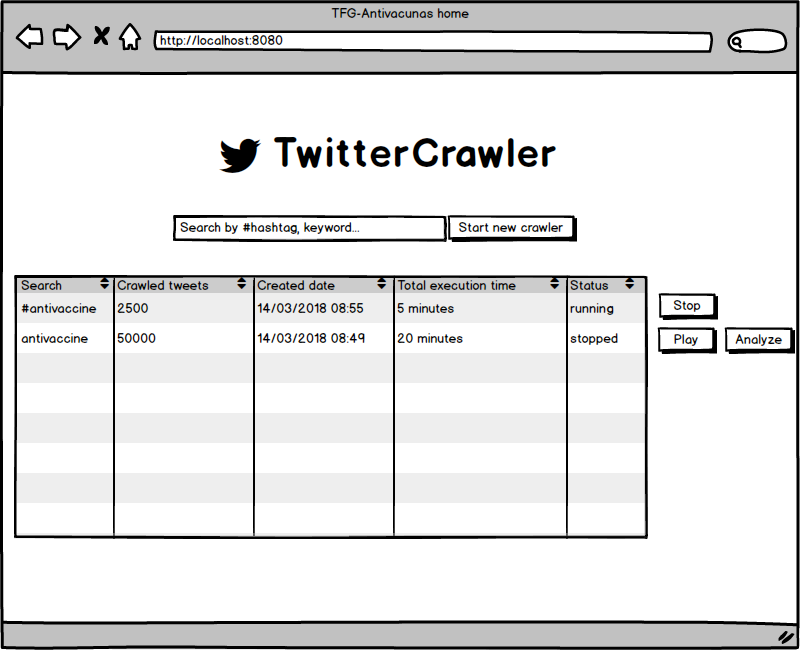
\includegraphics[width=60mm]{interfaz/03-15/1.png}}
\subfigure[\textit{Twitter} análisis]{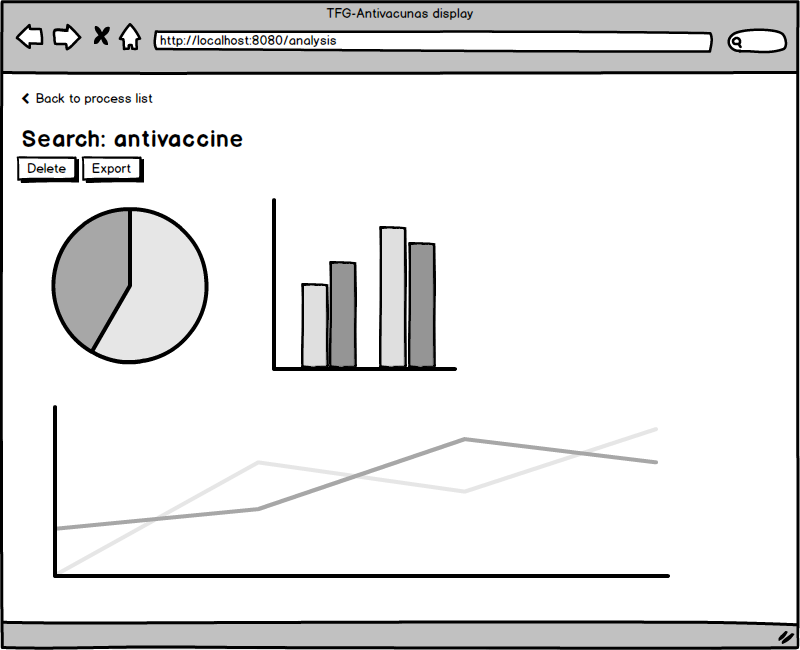
\includegraphics[width=60mm]{interfaz/03-15/2.png}}
\caption{Propuesta inicial interfaz de usuario}
\end{figure}
\pagebreak 

\noindent\textbf{Segunda propuesta presentada el 05/04/2018:}

\begin{figure}[H]
\centering
\subfigure[\textit{YouTube} búsqueda textual]{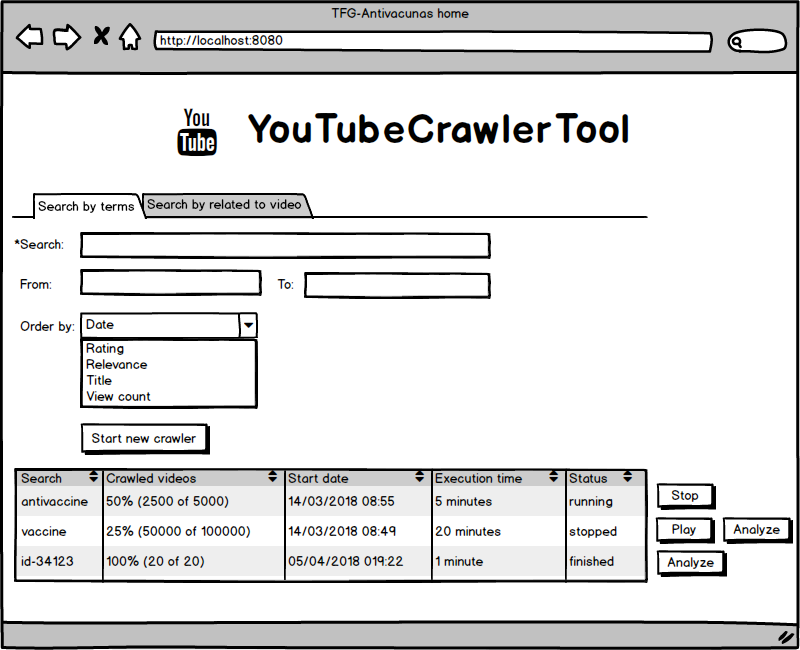
\includegraphics[width=60mm]{interfaz/04-05/1.png}}
\subfigure[\textit{YouTube} análisis textual]{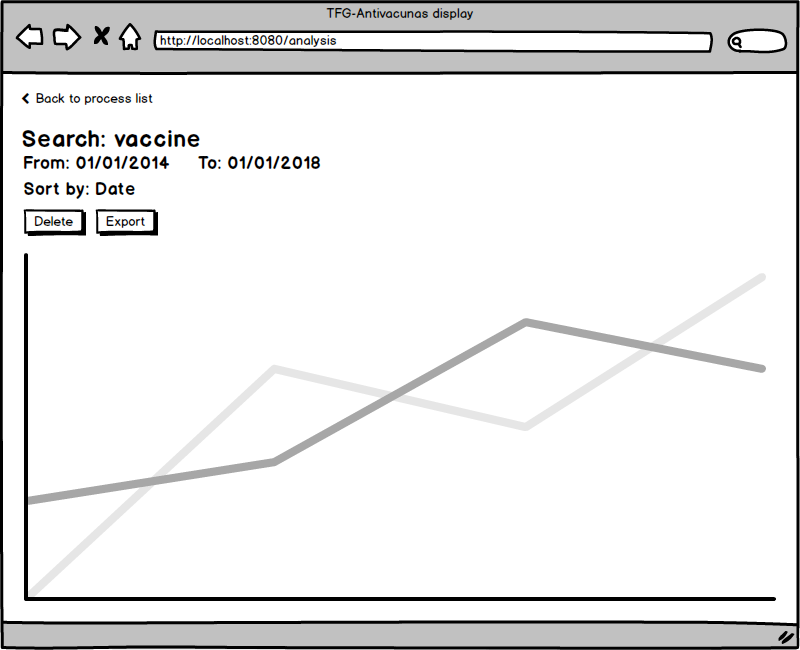
\includegraphics[width=60mm]{interfaz/04-05/2.png}}
\subfigure[\textit{YouTube} búsqueda vídeo relacionado]{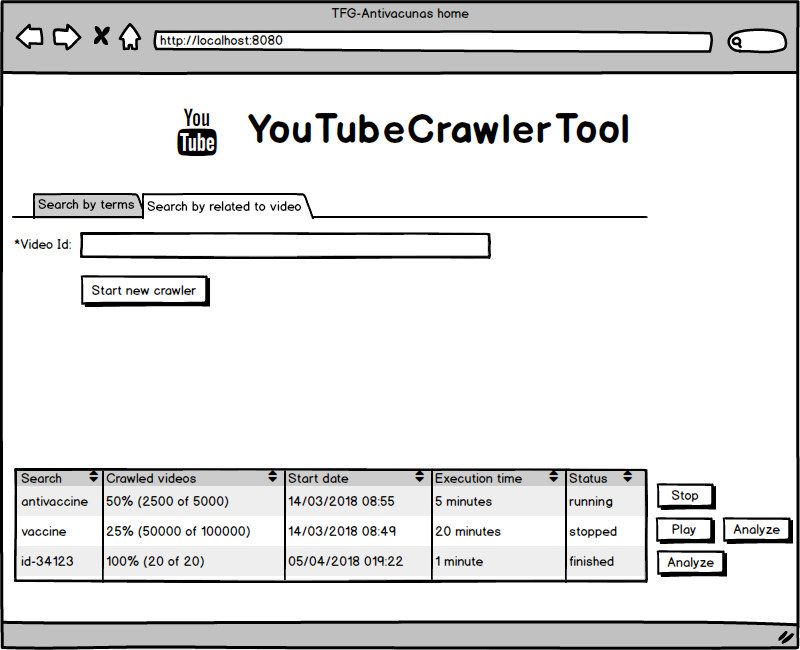
\includegraphics[width=60mm]{interfaz/04-05/3.png}}
\subfigure[\textit{YouTube} análisis vídeo relacionado]{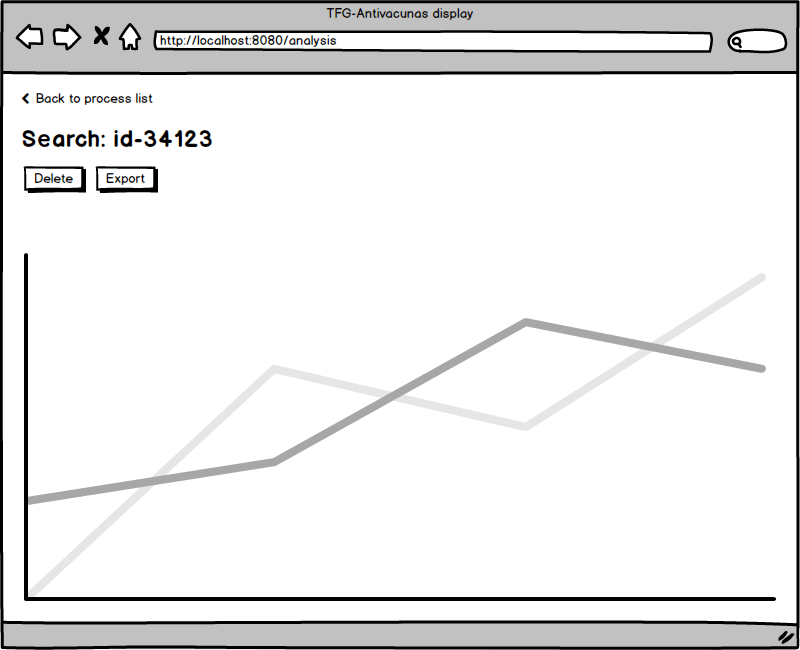
\includegraphics[width=60mm]{interfaz/04-05/4.png}}
\caption{Segunda propuesta interfaz de usuario}
\end{figure}

\noindent\textbf{Tercera y ultima propuesta presentada el 15/04/2018:}

\begin{figure}[H]
\centering
\subfigure[Login]{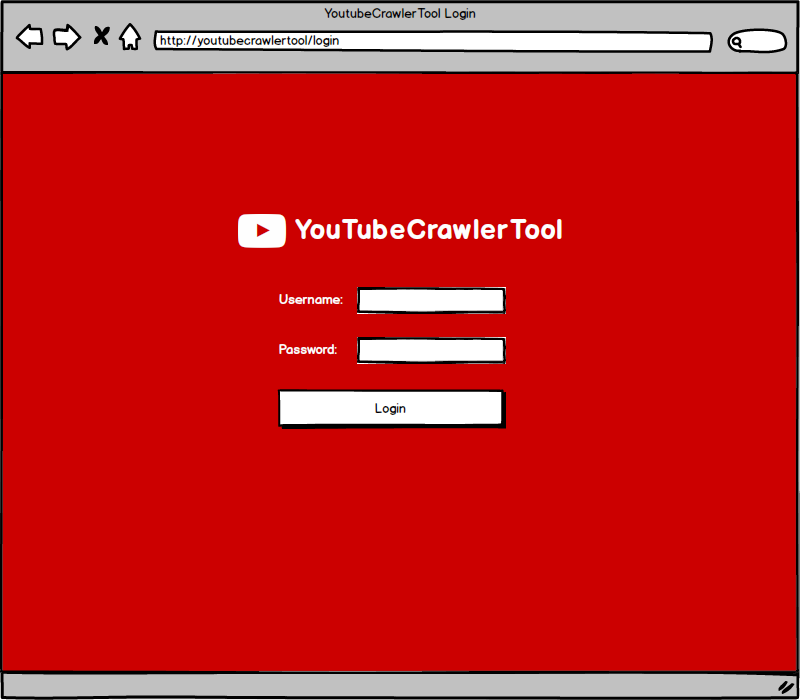
\includegraphics[width=60mm]{interfaz/04-15/1.png}}
\subfigure[Procesos de recolección]{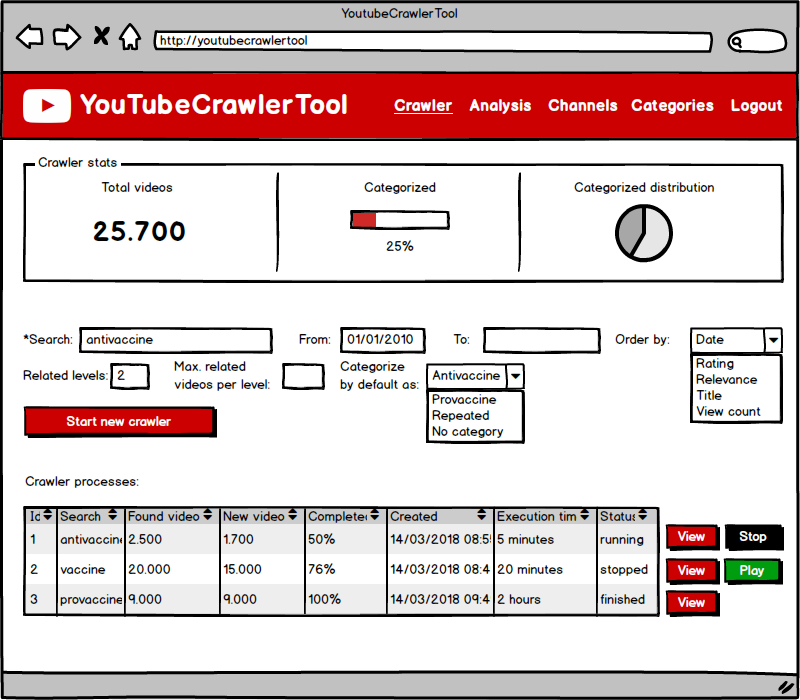
\includegraphics[width=60mm]{interfaz/04-15/2.png}}
\end{figure}
\begin{figure}[H]
\centering
\subfigure[Proceso de recolección]{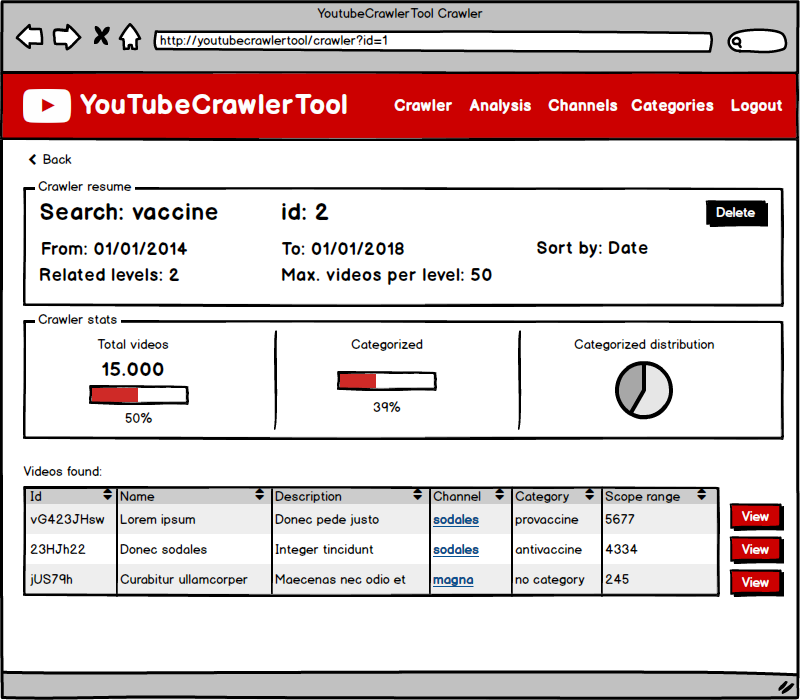
\includegraphics[width=60mm]{interfaz/04-15/3.png}}
\subfigure[Vista vídeo en detalle]{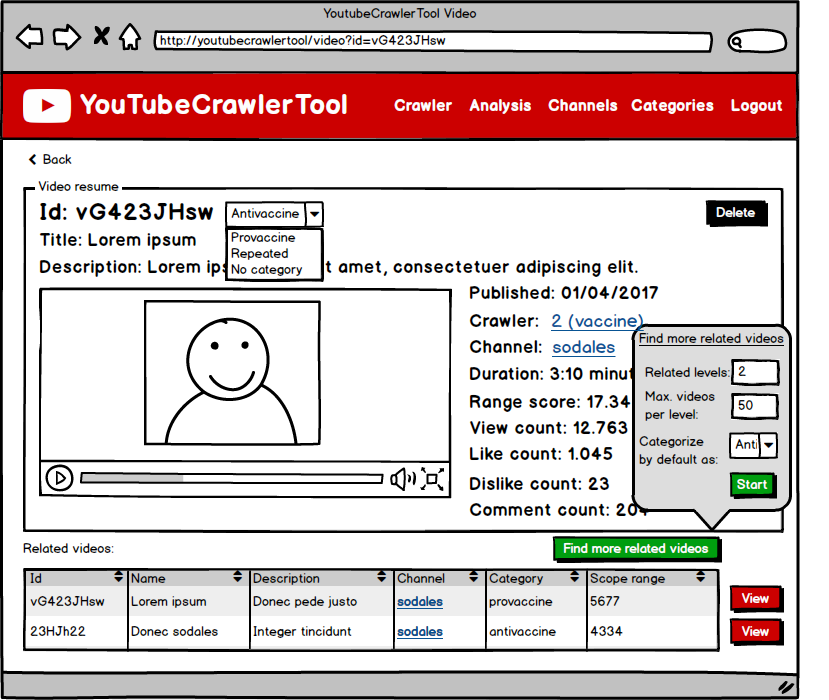
\includegraphics[width=60mm]{interfaz/04-15/4.png}}
\end{figure}
\begin{figure}[H]
\centering
\subfigure[Listado de canales]{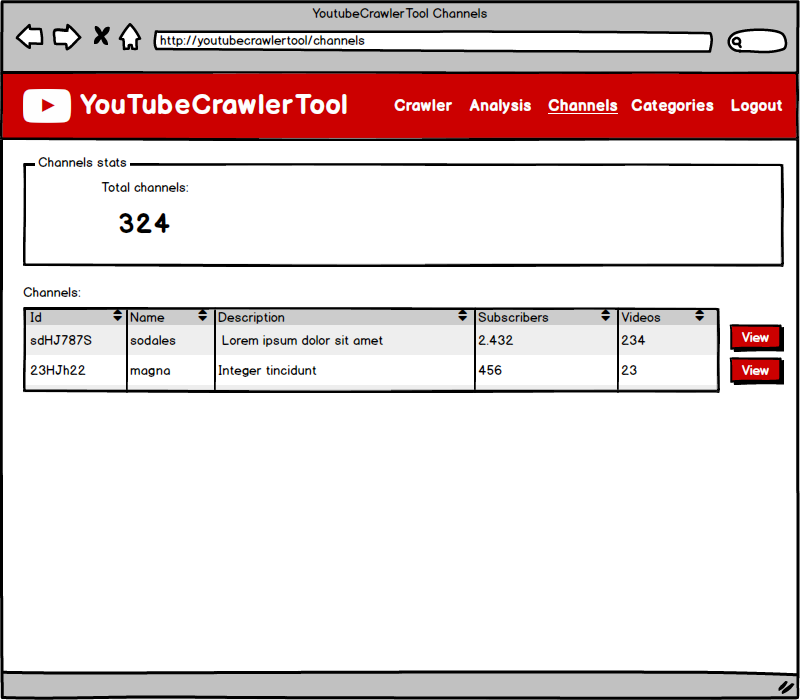
\includegraphics[width=60mm]{interfaz/04-15/5.png}}
\subfigure[Vista canal en detalle]{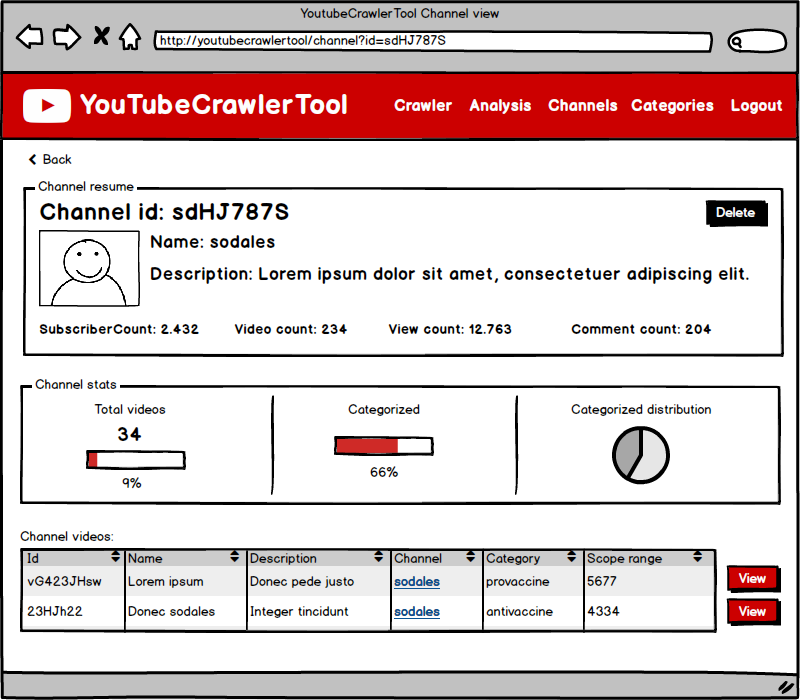
\includegraphics[width=60mm]{interfaz/04-15/6.png}}
\end{figure}
\begin{figure}[H]
\centering
\subfigure[Listado de categorías]{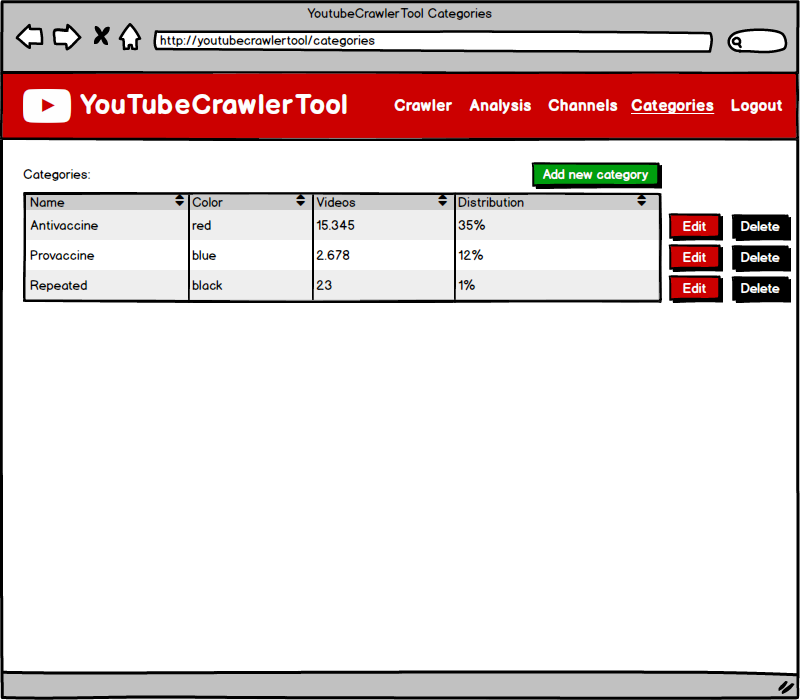
\includegraphics[width=60mm]{interfaz/04-15/7.png}}
\subfigure[Añadir nueva categoría]{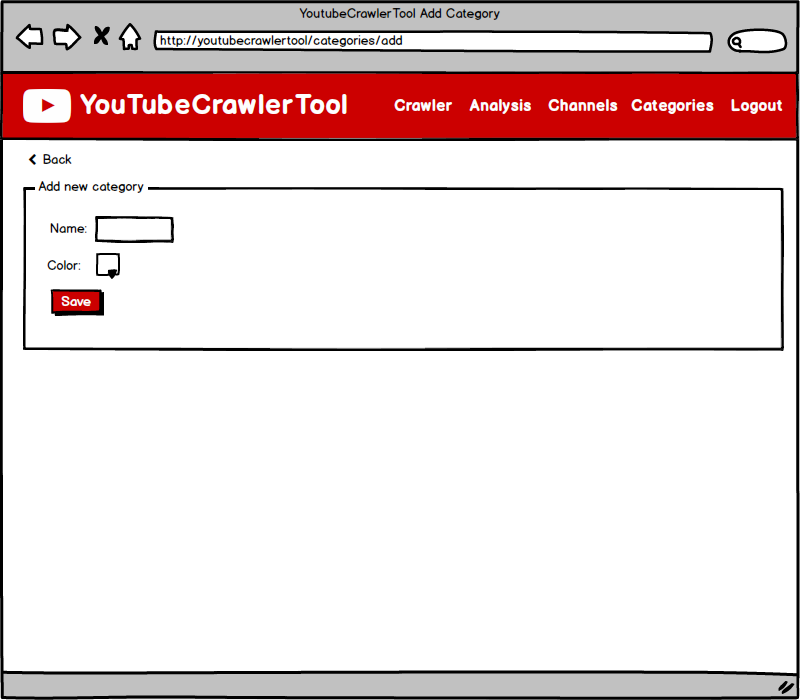
\includegraphics[width=60mm]{interfaz/04-15/8.png}}
\end{figure}
\begin{figure}[H]
\centering
\subfigure[Editar categoría]{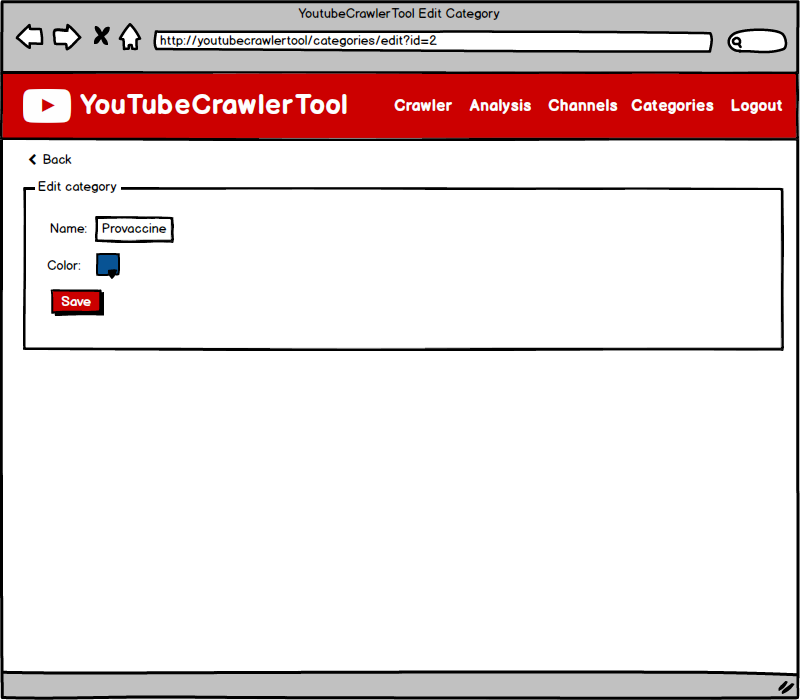
\includegraphics[width=60mm]{interfaz/04-15/9.png}}
\subfigure[Vista de análisis]{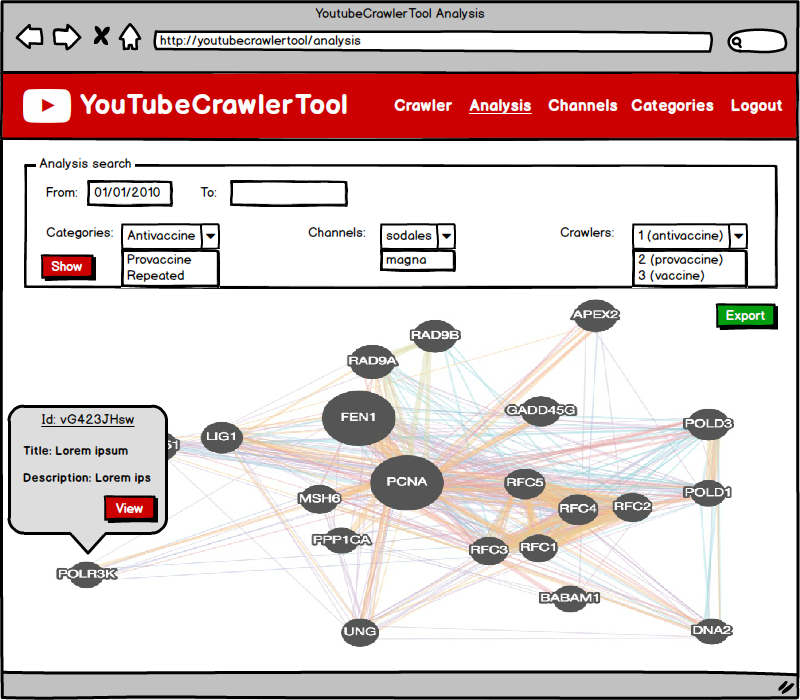
\includegraphics[width=60mm]{interfaz/04-15/10.png}}
\caption{Tercera y ultima propuesta de interfaz de usuario}
\end{figure}

Cabe destacar que, debido a iteraciones de desarrollo realizadas posteriormente a la presentación y aprobación de la ultima propuesta de interfaz de usuario presentada, esta no refleja el estado final de la aplicación.
\bigskip 

\subsection{Arquitectura WEB}
La decisión de realizar una aplicación Web viene motivada por las ventajas que aporta este medio en comparación con las aplicaciones de escritorio como por ejemplo, facilidades el trabajo colaborativo o centralizar la información y los procesos entre otros. Y de entre las diferentes arquitecturas Web, para el desarrollo del proyecto se escogió implementar una arquitectura REST por capas.
\\

REST (proveniente del acrónimo en ingles \textit{REpresentation State Transfer}) es un estilo arquitectónico en el desarrollo de aplicaciones Web que esta definido por una serie de principios. Algunos de los mas destacados son:
\begin{itemize}
\item Las solicitudes son sin estado.
\item Se sirven recursos, no funcionalidades (tales como objectos de base de datos).
\item Se accede a los recursos mediante URI que debe ser única por recurso.
\item Las operaciones sobre los recursos se realizan mediante HTTP especificando métodos estándar (tales como  \textit{GET}, \textit{PUT}, \textit{POST} y \textit{DELETE}).
\item Como formato para el intercambio de recursos se suele utilizar JSON o XML. 
\end{itemize}

La elección de esta arquitectura es a razón de los beneficios inherentes que aporta, tales como simplicidad en la arquitectura, escalable, extensible o la separación entre la capa de aplicación y capa de presentación. Gracias a esta arquitectura y de ser requerido en el futuro, ademas de disponer de un cliente Web como el diseñado en el proyecto actual, también seria factible, por ejemplo, proveer una aplicación móvil nativa sin tener que cambiar los servicios ofrecidos por el sistema.
\\

Como alternativa al uso de REST se considero utilizar una arquitectura basada en RPC. La gran diferencia entre ambas (entre otras) reside en el hecho que REST se centra en recursos mientras que RPC en funcionalidades. Por facilidad de uso y simplicidad se escogió implementar una arquitectura REST en detrimento de RPC.
\\

La aplicación de los principios REST conllevo a realizar otra decisión arquitectónica, dividir la aplicación por capas. En este caso, se escogió aplicar una arquitectura cliente-servidor de tres capas divididas en: 
\begin{itemize}
\item \textbf{Capa de datos}: Donde se persistirá la información de la aplicación utilizando un SGBD.
\item \textbf{Capa de aplicación}: En donde se llevara a cabo el acceso a datos, la lógica de negocio y de presentación que, a la vez, estará dividida entre el controlador de solicitudes de navegador (vistas HTML) y el controlador de solicitudes de recursos (API REST).
\item \textbf{Capa cliente}: Consistente en una interfaz de usuario web.
\end{itemize}

\begin{figure}[H]
\centering
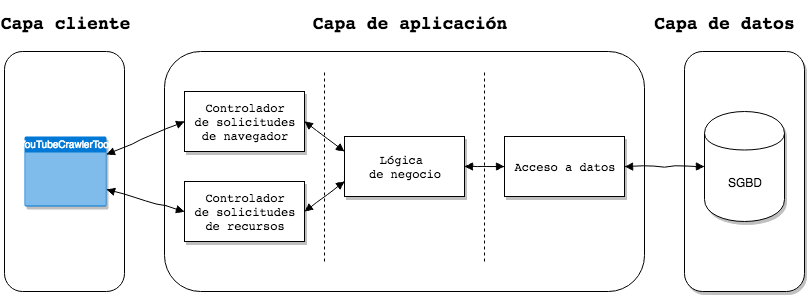
\includegraphics[scale=0.40]{diseno/ArquitecturaRESTPorCapas.png}
\caption{Arquitectura REST por capas}
\end{figure}

Gracias a esta distribución, se espera poder atorgar a la aplicación de una gran capacidad de reutilización y extensibilidad. En lo que ha distribución física se refiere, la capa cliente se ejecutara en los clientes Web de los usuarios y la capa de aplicación y de datos en un servidor. En los siguientes capítulos se detalla el diseño realizado para cada una de las capas.
\medskip 

\subsection{Diseño capa de datos}

\begin{figure}[H]
\centering
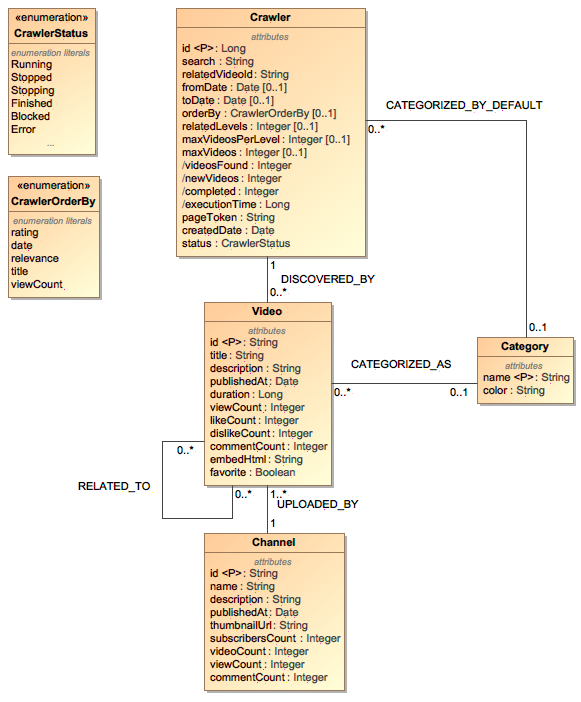
\includegraphics[scale=0.6]{diseno/DatabaseUML.png}
\caption{Diagrama de classes UML capa de datos}
\end{figure}

\medskip 

\subsection{Diseño capa de aplicación}

\begin{figure}[H]
\centering
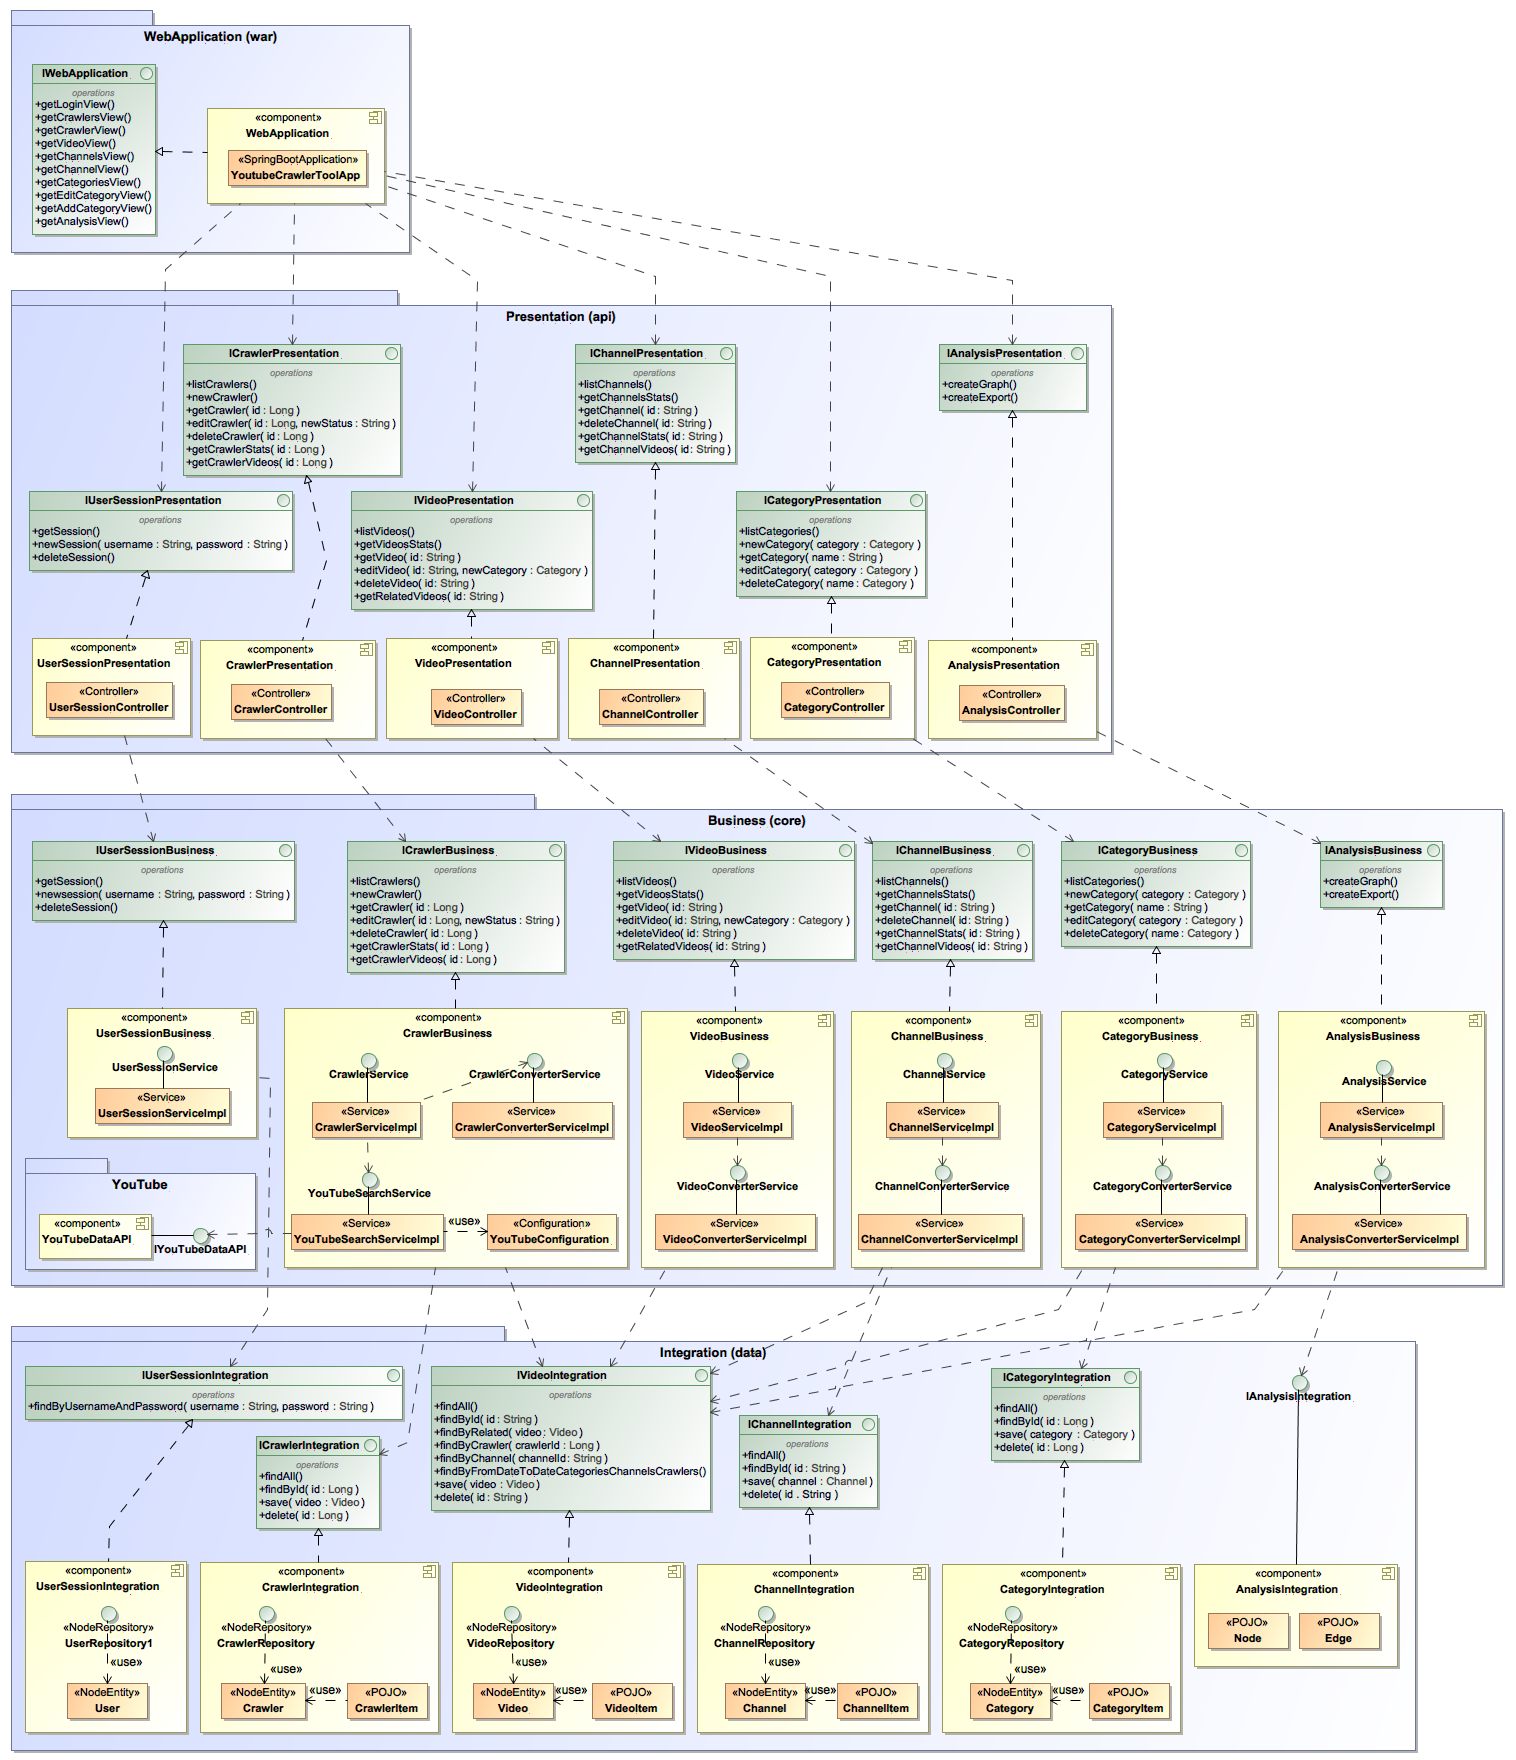
\includegraphics[scale=0.25]{diseno/ComponentDiagram3.png}
\caption{Diagrama de componentes}
\end{figure}

\medskip 

\subsubsection{Capa de acceso a datos}

\begin{figure}[H]
\centering
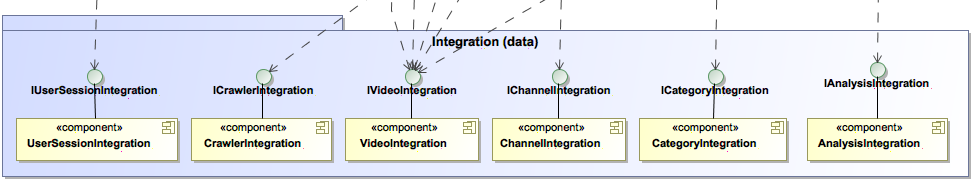
\includegraphics[scale=0.35]{diseno/accesoDatos/ComponentsDiagram.png}
\caption{Diagrama de componentes capa acceso a datos - v1}
\end{figure}

\begin{figure}[H]
\centering
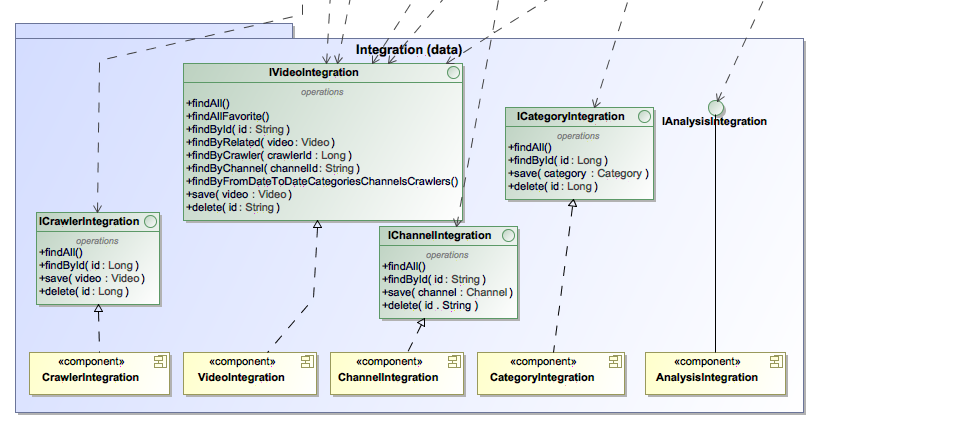
\includegraphics[scale=0.3]{diseno/accesoDatos/ComponentDiagram2.png}
\caption{Diagrama de componentes capa acceso a datos - v2}
\end{figure}

\begin{figure}[H]
\centering
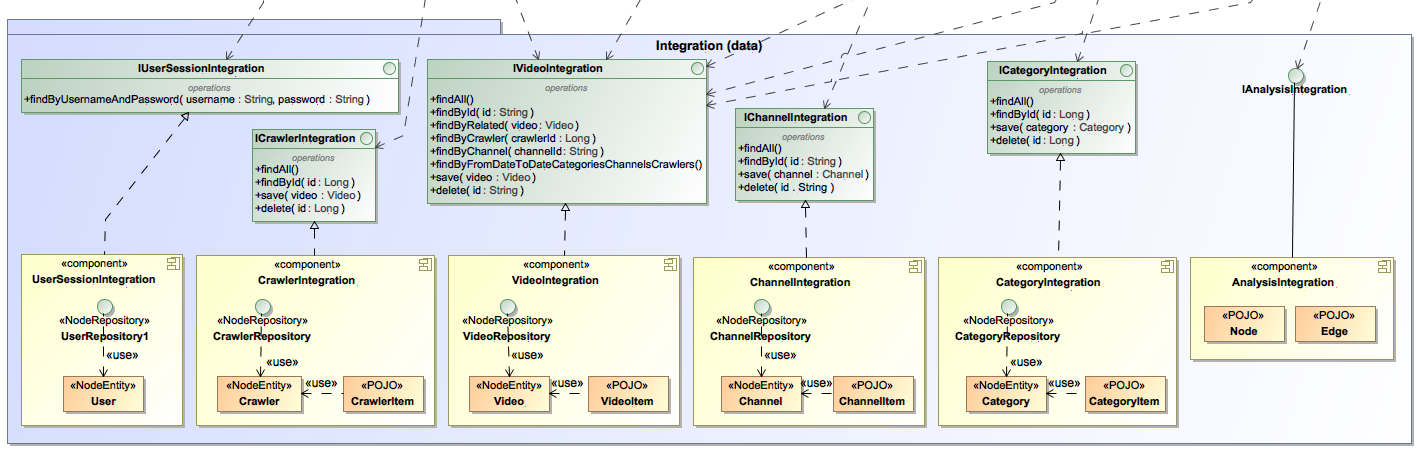
\includegraphics[scale=0.25]{diseno/accesoDatos/ComponentDiagram3.png}
\caption{Diagrama de componentes capa acceso a datos - v3}
\end{figure}

\medskip 

\subsubsection{Capa de lógica de negocio}

\begin{figure}[H]
\centering
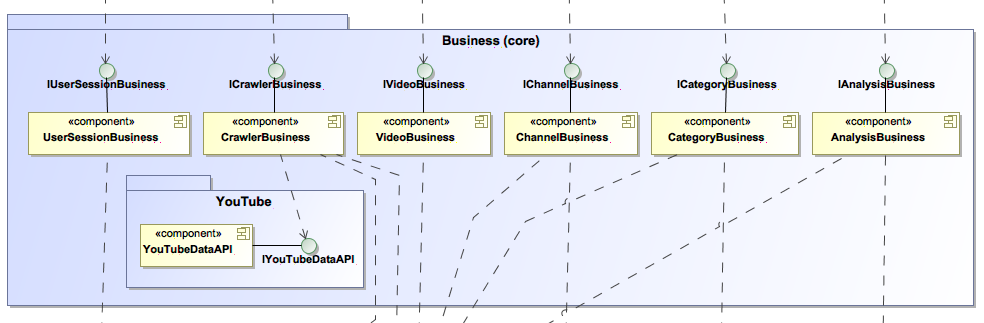
\includegraphics[scale=0.35]{diseno/negocio/ComponentsDiagram.png}
\caption{Diagrama de componentes capa de lógica de negocio - v1}
\end{figure}

\begin{figure}[H]
\centering
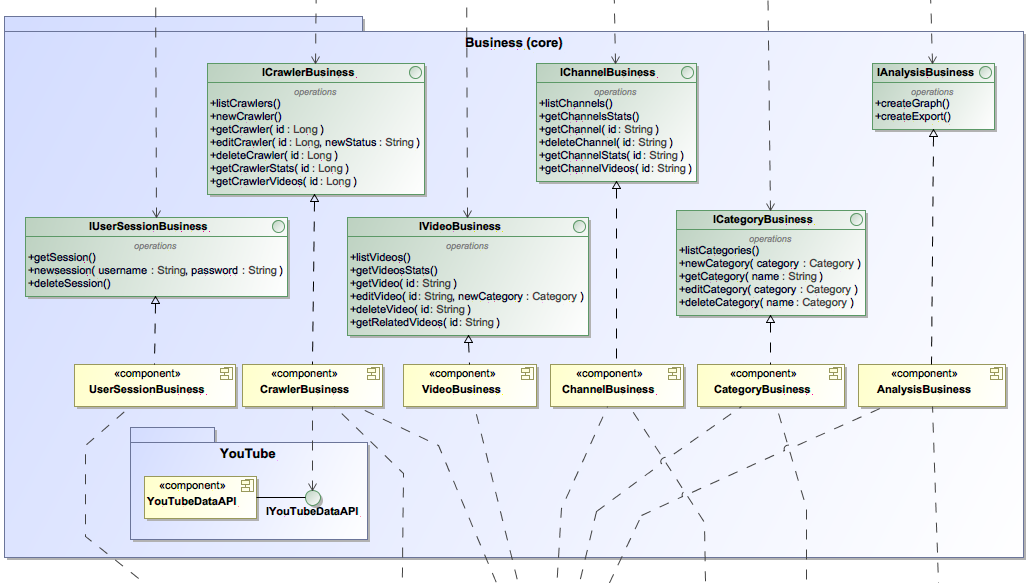
\includegraphics[scale=0.3]{diseno/negocio/ComponentDiagram2.png}
\caption{Diagrama de componentes capa de lógica de negocio - v2}
\end{figure}

\begin{figure}[H]
\centering
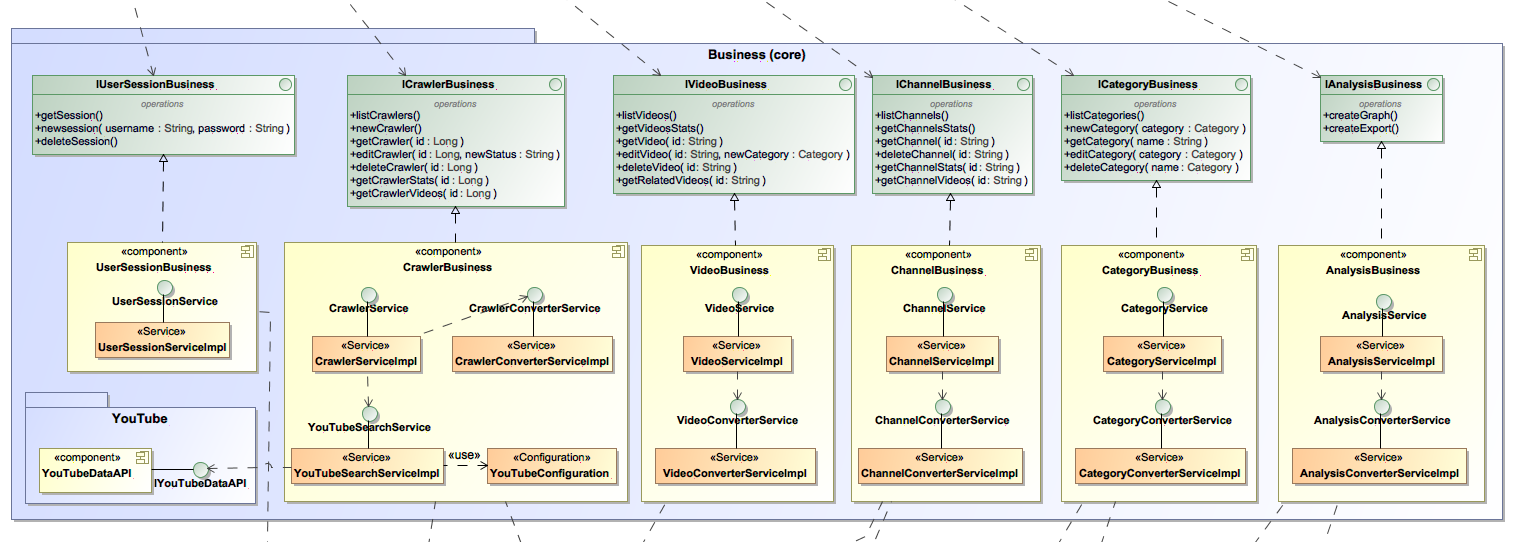
\includegraphics[scale=0.25]{diseno/negocio/ComponentDiagram3.png}
\caption{Diagrama de componentes capa de lógica de negocio - v3}
\end{figure}

\medskip 

\subsubsection{Capa de presentación}

\begin{figure}[H]
\centering
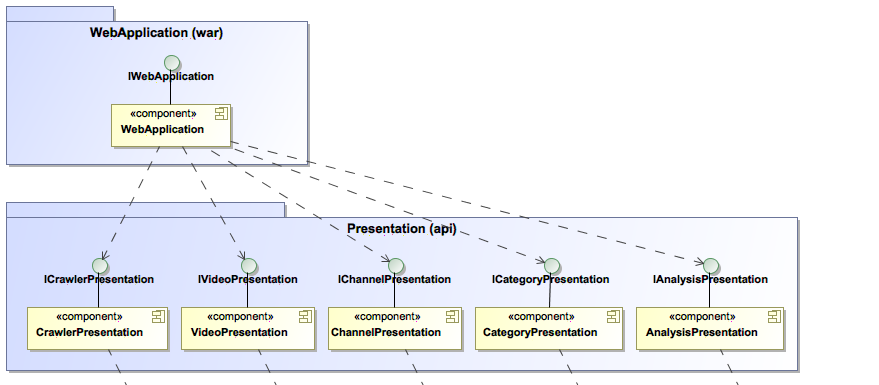
\includegraphics[scale=0.35]{diseno/presentacion/ComponentsDiagram.png}
\caption{Diagrama de componentes capa de presentación - v1}
\end{figure}

\begin{figure}[H]
\centering
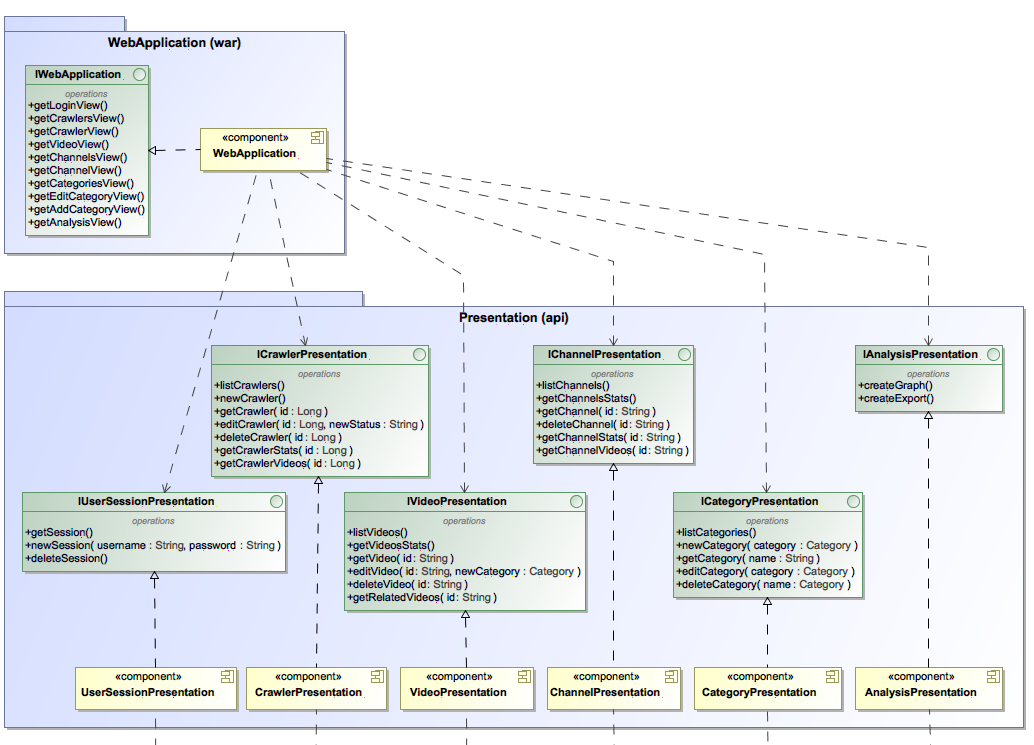
\includegraphics[scale=0.3]{diseno/presentacion/ComponentDiagram2.png}
\caption{Diagrama de componentes capa de presentación - v2}
\end{figure}

\begin{figure}[H]
\centering
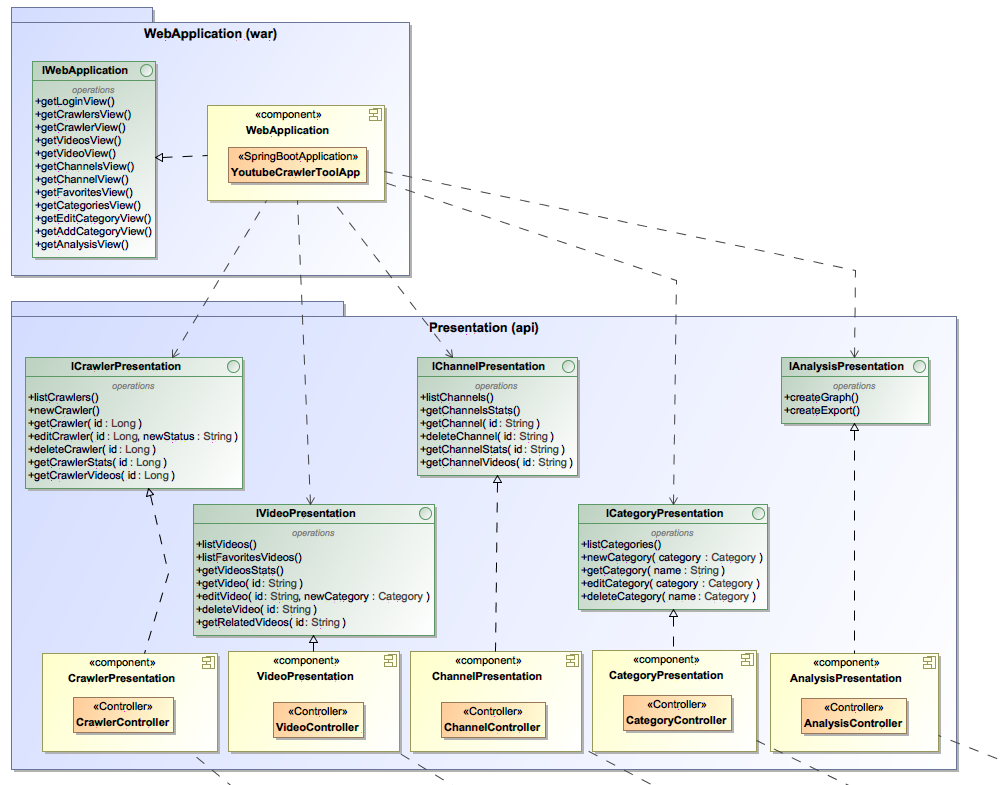
\includegraphics[scale=0.25]{diseno/presentacion/ComponentDiagram3.png}
\caption{Diagrama de componentes capa de presentación - v3}
\end{figure}

\noindent\textbf{Componente \textit{crawler}:}

\begin{table}[H]
\centering
\resizebox{\textwidth}{!}{%
\begin{tabular}{|l|l|l|}
\hline
\textbf{Metodo} & \textbf{Uri}            & \textbf{Descripción}                                               \\ \hline
GET             & api/crawlers               & Lista todos los procesos de recolección.                           \\ \hline
POST            & api/crawlers               & Inicia un nuevo proceso de recolección. Requiere autentificación.  \\ \hline
GET             & api/crawlers/\{id\}        & Devuelve un proceso de recolección.                                \\ \hline
PUT             & api/crawlers/\{id\}        & Editar un proceso de recolección. Requiere identificación.        \\ \hline
DELETE          & api/crawlers/\{id\}        & Borra un proceso de recolección. Requiere identificación.         \\ \hline
GET             & api/crawlers/\{id\}/stats  & Devuelve las estadísticas de un proceso de recolección.            \\ \hline
GET             & api/crawlers/\{id\}/videos & Lista todos los vídeos descubiertos por un proceso de recolección. \\ \hline
\end{tabular}%
}
\caption{Componente \textit{crawler} API}
\end{table}

\noindent\textbf{Componente \textit{video}:}
\begin{table}[H]
\centering
\resizebox{\textwidth}{!}{%
\begin{tabular}{|l|l|l|}
\hline
\textbf{Metodo} & \textbf{Uri}             & \textbf{Descripción}                              \\ \hline
GET             & api/videos               & Lista todos los vídeos.                           \\ \hline
GET             & api/videos/stats         & Devuelve las estadísticas de todos los vídeos.    \\ \hline
GET             & api/videos/favorites     & Devuelve los vídeos favoritos.                    \\ \hline
GET             & api/videos/\{id\}        & Devuelve un vídeo.                                \\ \hline
PUT             & api/videos/\{id\}        & Editar un vídeo. Requiere identificación.         \\ \hline
DELETE          & api/videos/\{id\}        & Borra un vídeo. Requiere identificación.          \\ \hline
GET             & api/videos/\{id\}/videos & Lista todos los vídeos relacionados con un vídeo. \\ \hline
\end{tabular}%
}
\caption{Componente \textit{video} API}
\end{table}

\noindent\textbf{Componente \textit{channel}:}
\begin{table}[H]
\centering
\resizebox{\textwidth}{!}{%
\begin{tabular}{|l|l|l|}
\hline
\textbf{Metodo} & \textbf{Uri}               & \textbf{Descripción}                              \\ \hline
GET             & api/channels               & Lista todos los canales                           \\ \hline
GET             & api/channels/\{id\}        & Devuelve un canal.                                \\ \hline
DELETE          & api/channels/\{id\}        & Borra un canal. Require identificación            \\ \hline
GET             & api/channels/\{id\}/stats  & Devuelve la estadisticas de un canal              \\ \hline
GET             & api/channels/\{id\}/videos & Lista todos los videos relacionados con un canal. \\ \hline
\end{tabular}%
}
\caption{Componente \textit{channel} API}
\end{table}

\noindent\textbf{Componente \textit{category}:}
\begin{table}[H]
\centering
\resizebox{\textwidth}{!}{%
\begin{tabular}{|l|l|l|}
\hline
\textbf{Metodo} & \textbf{Uri}                   & \textbf{Descripción}                                    \\ \hline
GET             & api/categories                 & Lista todas las categorías                              \\ \hline
POST            & api/categories                 & Crea una nueva categoría. Requiere identificación.      \\ \hline
GET             & api/categories/\{name\}        & Devuelve una categoría.                                 \\ \hline
PUT             & api/categories/\{name\}        & Editar una categoría. Requiere identificación.          \\ \hline
DELETE          & api/categories/\{name\}        & Borra una categoría.                                    \\ \hline
GET             & api/categories/\{name\}/stats  & Devuelve las estadísticas de una categoría.             \\ \hline
GET             & api/categories/\{name\}/videos & Lista todos los vídeos categorizados por una categoría. \\ \hline
\end{tabular}%
}
\caption{Componente \textit{category} API}
\end{table}

\noindent\textbf{Componente \textit{analysis}:}
\begin{table}[H]
\centering
\resizebox{\textwidth}{!}{%
\begin{tabular}{|l|l|l|}
\hline
\textbf{Metodo} & \textbf{Uri} & \textbf{Descripción}                                           \\ \hline
POST            & api/graphs   & Crea un nuevo grafo (no se persiste, se muestra por pantalla). \\ \hline
\end{tabular}%
}
\caption{Componente \textit{analysis} API}
\end{table}

\medskip 

\subsection{Diseño capa cliente}
// Explicar combinación jsp mas llamadas Ajax desde javascript

\begin{figure}[H]
\centering
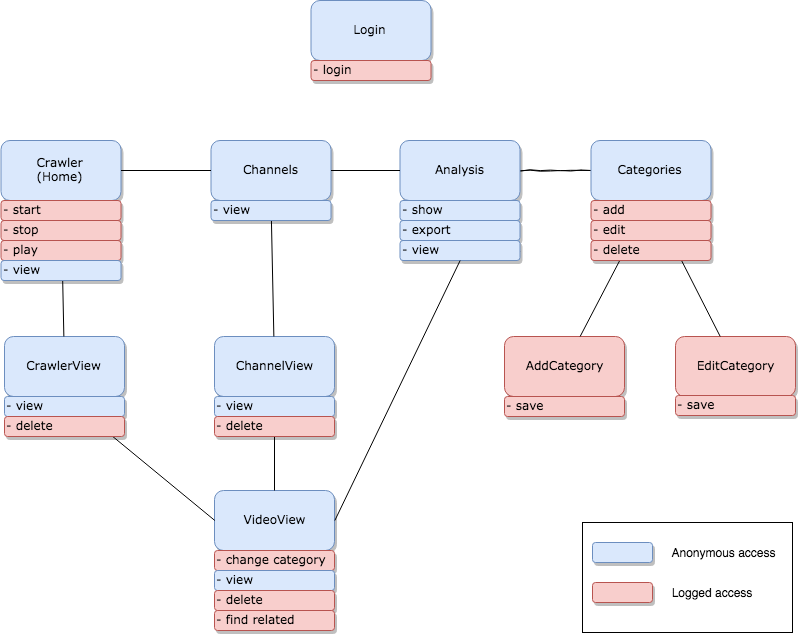
\includegraphics[scale=0.25]{diseno/capaCliente.png}
\caption{Diseño vistas capa cliente}
\end{figure}

\newpage 




\section{Desarrollo}
\bigskip

//TODO: Hablar de patrones usados (factory y etc) y framworks utilizados
\subsection{Entorno de desarrollo}
Aplicación web (con POCYouTubeCrawlerNeo4j instalado):
\url{http://youtubecrawlertoolwebapp.azurewebsites.net} 

Servidor base de datos Neo4j:
\url{http://51.136.48.142:7474/browser} 
Usuario: neo4j
Password: Y01t1b3cr4wl3rt00l
Consulta de ejemplo: MATCH (n) RETURN n
\medskip 

\subsection{Pruebas de concepto}
\begin{itemize}
\item \textbf{Twitter crawler:} \url{https://github.com/jsanchezmend/TFGAntivacunas/tree/master/POCTwitterCrawler}
\item \textbf{YouTube crawler:} \url{https://github.com/jsanchezmend/TFGAntivacunas/tree/master/POCYouTubeCrawler}
\item \textbf{Visualización en grafo:}: \url{https://github.com/jsanchezmend/TFGAntivacunas/tree/master/POCYouTubeCrawler}
\item \textbf{Neo4j:} \url{https://github.com/jsanchezmend/TFGAntivacunas/tree/master/POCYouTubeCrawlerNeo4j}
\end{itemize}
\medskip 

\subsubsection{POCTwitterCrawler}
\medskip 

\subsubsection{POCYouTubeCrawler}
\medskip 

\subsubsection{POCYouTubeCrawlerNeo4j}
\medskip 

\subsection{Análisis YouTube Data API}\label{youTubeDataAPI} 
\medskip 

\subsection{Elección de Neo4j como SGBD}
\medskip 

\subsection{Estructura de la aplicación}
\medskip 

\subsection{Acceso a datos}
// Spring data, entities, repositorios y POJOS
\medskip 

\subsection{Crawler de YouTube}
// Explicar conexión con YouTube y como se ha implementado el crawler
\medskip 

\subsection{Visualización de vídeos en grafo}
// Busqueda de videos y su representación en grafo Cytripode.js
\medskip 

\subsection{Otras funcionalidades}
// Accose a videos, favoritos, canales, etc.. 
\medskip 

\subsection{Capa de seguridad}
//Spring security
\medskip 

\subsection{Capa de presentación}
//Plantillas JSP con Themleaf y requests Ajax con Jquery y jquery para modificar el dom
\medskip 

\subsection{Definición y ejecución de pruebas}
\newpage 





\section{Implementación y puesta en funcionamiento}
\bigskip 

\subsection{Manual de instalación y requerimientos}
\medskip 

\subsection{Servidor de explotación}
\medskip 

\subsection{Formación y sensibilización}
\medskip 

\subsection{Funcionalidades no implementadas}
// Stats
\medskip 

\subsection{Propuesta de mejoras}
//API error handling, mejores logs, mas filtros de analisis y por base de datos, performance del grafo, UI en general, accesibilidad y usabilidad. inteligencia artificial para categorizar automaticamente los videos uilizando, por ejemplo, un modelo baso en reglas.
\newpage 




\section{Conclusiones}
\bigskip 

Este capítulo tiene que incluir:
\begin{itemize}
\item Una descripción de las conclusiones del trabajo: Qué lecciones se han aprendido del trabajo?.
\item Una reflexión crítica sobre el logro de los objetivos planteados inicialmente: Hemos logrado todos los objetivos? Si la respuesta es negativa, por qué motivo? 
\item Un análisis crítico del seguimiento de la planificación y metodología a lo largo del producto: Se ha seguido la planificación? La metodología prevista ha sido la adecuada? Ha habido que introducir cambios para garantizar el éxito del trabajo? Por qué? 
\item Las líneas de trabajo futuro que no se han podido explorar en este trabajo y han quedado pendientes.
\end{itemize}

\subsection{Conclusiones del trabajo}
// mencionar conclusiones de Johanna
// Puntos fuertes y debiles
// Criticas dificultades
// ha merecido la pena etc...
\medskip 

\subsection{Grado de cumplimiento de los objetivos}
\medskip 

\subsection{Seguimiento de la planificación y metodología}\label{sec:seguiminetoPlanificacion}
//TODO: Gant tentativo vs gant final (tomar prestado de los informes de seguimiento)
\medskip 

\subsection{Opinión del proyecto}
\newpage 


\section{Glosario}
\bigskip

Definición de los términos y acrónimos más relevantes utilizados dentro de la Memoria. 
\newpage 


\section{Bibliografía}
\bigskip

\begin{thebibliography}{0}
  \bibitem{1} \url{https://es.wikipedia.org/wiki/Controversia_de_las_vacunas} (07/03/2018)
  \bibitem{2} \url{http://www.elmundo.es/cataluna/2015/06/27/558e5fb2e2704ea41e8b4576.html} (07/03/2018)
  \bibitem{3} \url{https://buenavibra.es/movida-sana/salud/italia-sarampion-movimientos-antivacunas} (16/03/2018)
  \bibitem{4} \url{https://es.wikipedia.org/wiki/Ciencia_de_datos} (07/03/2018)
  \bibitem{5} \url{https://es.wikipedia.org/wiki/Interfaz_de_programacion_de_aplicaciones} (07/03/2018)
  \bibitem{6} \url{https://es.wikipedia.org/wiki/NoSQL} (07/03/2018)
  \bibitem{7} \url{https://es.wikipedia.org/wiki/Macrodatos} (07/03/2018)
  \bibitem{8} \url{https://es.wikipedia.org/wiki/Scrum_(desarrollo_de_software)} (16/03/2018)
  \bibitem{9} \url{https://trello.com} (16/03/2018)
  \bibitem{10} \url{http://www.oracle.com/technetwork/java/index.html} (23/05/2018)
  \bibitem{11} \url{https://spring.io/} (23/05/2018)
  \bibitem{12} \url{https://es.wikipedia.org/wiki/JavaScript} (23/05/2018)
  \bibitem{13} \url{https://jquery.com/} (23/05/2018)
  \bibitem{14} \url{https://es.wikipedia.org/wiki/Base_de_datos_orientada_a_grafos} (23/05/2018)
  \bibitem{15} \url{https://es.wikipedia.org/wiki/Dise%C3%B1o_centrado_en_el_usuario} (24/05/2018)
  \bibitem{16} \url{https://es.wikipedia.org/wiki/Caso_de_uso} (24/05/2018) 
  \bibitem{17} \url{https://developer.twitter.com/en/docs/tweets/search/overview} (26/05/2018) 
  \bibitem{18} \url{https://developers.google.com/youtube/v3/getting-started?hl=es-419#quota} (26/05/2018) 
\end{thebibliography}
\newpage 


\section{Anexos}
\bigskip

Listado de apartados que son demasiado extensos para incluir dentro de la memoria y tienen un carácter autocontienido (por ejemplo, manuales de usuario, manuales de instalación, etc.) 

Dependiente del tipo de trabajo, es posible que no haya que añadir ningún anexo.

\end{document}
